\documentclass[10pt,letterpaper]{book}


%\usepackage[left=4cm, width=15.50cm, height=23.00cm]{geometry}
\usepackage[width=15.50cm, height=23.00cm]{geometry}
\usepackage[english]{babel}
\usepackage[utf8]{inputenc}
\usepackage[T1]{fontenc}
\usepackage{dsfont}
\usepackage{amsmath}
\usepackage{amsfonts}
\usepackage{amssymb}
\usepackage{graphicx}
\usepackage{paracol}
\usepackage{xparse}
\usepackage{sidecap}
\usepackage[makeroom]{cancel}
\usepackage{capt-of}
\usepackage[margin=1cm]{caption}
\usepackage[dvipsnames]{xcolor}
\usepackage{xpatch}
\usepackage{subcaption}
\usepackage[most]{tcolorbox}
\usepackage{lipsum}
\usepackage{float}
\usepackage{imakeidx}
\usepackage{wrapfig}
\usepackage{marginnote}
\usepackage{ upgreek }
\usepackage{bm}
\usepackage{enumerate}
\usepackage{mathrsfs} 
\usepackage{array}
\usepackage{arydshln}
\usepackage{hyperref}

\graphicspath{{Images/}}


\makeindex[columns=3, title=Indice Analitico, intoc]

\newcolumntype{M}[1]{>{\centering\arraybackslash}m{#1}}
\captionsetup{font = {it, small}, labelfont={color=NavyBlue, bf}}



\newcommand{\F}{\mathscr F}
\newcommand{\four}[1]{\mathscr{F}\left\{ #1 \right\}}
\newcommand{\antifour}[1]{\mathscr{F}^{-1}\left\{ #1 \right\}}
\newcommand{\prob}[1]{\textrm{Pr}\left\{ #1 \right\}}
\newcommand{\intinf}{\int_{-\infty}^\infty}
\newcommand{\infsum}[1]{\sum_{#1=-\infty}^\infty}
\newcommand{\sinc}{\textrm{sinc}}
\newcommand{\rect}{\textrm{rect}}
\renewcommand{\Re}[1]{\textrm{Re}\left\{ #1 \right\}}
\renewcommand{\Im}[1]{\textrm{Im}\left\{ #1 \right\}}
\newcommand{\dft}{discrete Fourier transform }
\newcommand{\fft}{fast Fourier transform }
\newcommand{\circconv}[1]{\underset{\text{\tiny $#1$}} \otimes}
\newcommand{\Z}[1]{\mathcal{Z}\left\{#1\right\}}

\newcommand{\var}[1]{\textrm{Var}\{#1\}}
\newcommand{\dtft}{discrete-time Fourier transform }
\newcommand{\ctft}{continuous-time Fourier transform }

\newcommand{\de}[1]{\textbf{\textcolor{NavyBlue}{#1}}}

\newcommand{\figura}[5]{\begin{SCfigure}[#2][b!h!t!]
		\centering
		\includegraphics[width=#1 cm]{#3}
		\caption{#4} \label{#5}
\end{SCfigure}}





\newcommand{\bfcolor}[1]{\renewcommand*{\textbf}[1]{{\bfseries {\color{#1}##1}}}}
\newcommand{\tabrule}{\rule{\linewidth}{1pt}}

\setcolumnwidth{0.3\textwidth}


\newcounter{domande}
\refstepcounter{domande}
\newcommand{\newquestion}{\vspace{3mm} \noindent \rule{\linewidth}{2pt}\subsection*{Question \thedomande} \refstepcounter{domande}}



\newcounter{concetti}
\newenvironment{concetto}{
	
	\bfcolor{NavyBlue}
	\refstepcounter{concetti}
	{\color{NavyBlue}\textbf{Concetto \theconcetti:}} \quad
}{
}
\numberwithin{concetti}{chapter}
\tcolorboxenvironment{concetto}{
	boxrule=0pt,
	boxsep=0pt,
	colback={White!90!NavyBlue},
	enhanced jigsaw, 
	borderline west={2pt}{0pt}{NavyBlue},
	sharp corners,
	before skip=5pt,
	after skip=10pt,
	breakable,
}

\newcounter{teoremi}
\newenvironment{teorema}[2]{
	\bfcolor{ForestGreen}
	\refstepcounter{teoremi}
	\textbf{Concetto \theteoremi #1} 
	\vspace{3mm} 
	
	\texttt{Ipotesi: } #2
	
	\vspace{3mm} 
	
	\texttt{Enunciato}: 
}{
}
\numberwithin{teoremi}{chapter}
\tcolorboxenvironment{teorema}{
	boxrule=0pt,
	boxsep=0pt,
	colback={White!100!ForestGreen},
	enhanced jigsaw, 
	borderline west={2pt}{0pt}{ForestGreen},
	sharp corners,
	before skip=5pt,
	after skip=10pt,
	breakable,
}


\newenvironment{dimostrazione}{
	\bfcolor{Orchid}
	\textbf{Dimostrazione} \quad
}{ }
\tcolorboxenvironment{dimostrazione}{
	boxrule=0pt,
	boxsep=0pt,
	colback={White!100!NavyBlue},
	enhanced jigsaw, 
	borderline west={2pt}{0pt}{Orchid},
	sharp corners,
	before skip=5pt,
	after skip=10pt,
	breakable,
}

\newenvironment{osservazione}{
	\bfcolor{BurntOrange}
	\textbf{Osservazione: }
}{ }
\tcolorboxenvironment{osservazione}{
	boxrule=0pt,
	boxsep=0pt,
	colback={White!100!BurntOrange},
	enhanced jigsaw, 
	borderline west={2pt}{0pt}{BurntOrange},
	sharp corners,
	before skip=5pt,
	after skip=10pt,
	breakable,
}

\newenvironment{note}{
	\bfcolor{CadetBlue}
	\textbf{Note: }
}{ }
\tcolorboxenvironment{note}{
	boxrule=0pt,
	boxsep=0pt,
	colback={White!100!CadetBlue},
	enhanced jigsaw, 
	borderline west={2pt}{0pt}{CadetBlue},
	sharp corners,
	before skip=5pt,
	after skip=10pt,
	breakable,
}




\newenvironment{proof}{
	\noindent	
%	\renewcommand{\de}[1]{ { \color{ForestGreen} \textbf{#1} } }
	
	{\color{ForestGreen}\textbf{Proof:}}
}{
}
\tcolorboxenvironment{proof}{
	boxrule=0pt,
	boxsep=0pt,
%	colback={White!90!ForestGreen},
	enhanced jigsaw, 
	borderline west={2pt}{0pt}{ForestGreen},
	sharp corners,
	before skip=5pt,
	after skip=5pt,
	breakable,
}


\newcounter{exercises}
\numberwithin{exercises}{chapter}
\newenvironment{exercise}[1]{
	\bfcolor{Periwinkle}
	\noindent
	\refstepcounter{exercises}
	{\color{Periwinkle}\textbf{Exercise \theexercises#1}  } 
	\vspace{3mm}
	
	\noindent
}{
}


\tcolorboxenvironment{exercise}{
	boxrule=0pt,
	boxsep=0pt,
	colback={White!90!Periwinkle},
	enhanced jigsaw, 
	borderline west={2pt}{0pt}{Periwinkle},
	sharp corners,
	before skip=10pt,
	after skip=10pt,
	breakable,
}

\newcounter{examples}
\numberwithin{examples}{chapter}
\newenvironment{example}[1]{
	\bfcolor{Periwinkle}
	\noindent
	\refstepcounter{examples}
	{\color{Periwinkle}\textbf{Example \theexamples#1}  } 
	\vspace{3mm}
	
	\noindent
}{
}


\tcolorboxenvironment{example}{
	boxrule=0pt,
	boxsep=0pt,
	colback={White!90!Periwinkle},
	enhanced jigsaw, 
	borderline west={2pt}{0pt}{Periwinkle},
	sharp corners,
	before skip=10pt,
	after skip=10pt,
	breakable,
}

%\usepackage[defaultfam,light,tabular,lining]{montserrat}
%\renewcommand*\oldstylenums[1]{{\fontfamily{Montserrat-TOsF}\selectfont #1}}


\begin{document}
	
	\frontmatter
	
	\begin{center}
		\vspace{3cm}
		\thispagestyle{empty}
		
\includegraphics[width=5cm]{logouni}
		
		\vspace{1cm}
		\rule{5cm}{0.5pt}
		\vspace{1cm}		
		
		{\Large Università degli Studi di Trento}
		
		\vspace{2cm}
		{\Large Department of Industrial Engineering} \\ \vspace{2mm}
		{\LARGE \textbf{Digital Signal Processing for Mechatronics}} \\ \vspace{2mm}
		{\Large Prof.: Macii David}\\
		
		\vspace{2cm}
		{\LARGE \textbf{Course Notes}}
		
		\vspace{1cm}
		\rule{5cm}{0.5pt}
		\vspace{1cm}	
		
		{\large 
			Matteo Dalle Vedove \\
			\makeatletter
			matteo.dallevedove@studenti.unitn.it
			
			\vspace{2cm}
			Academic Year 2021-2022 \\ \today}
	\end{center}
	
	\tableofcontents
		
	\chapter{Introduction}

	\textbf{06/10/2021}
	
	\paragraph{Energy and power signals} Given a signal $x(t)$ with $t\in [-T/2, T/2]$ or a discrete one $x(n)$ with $n \in [-N/2,N/2]$, we define the \de{energy} $E_T$ and the \de{power} $P_T$ as
	\begin{equation}
	\begin{split}		
		E_T & = \int_{-T/2}^{T/2} |x(t)|^2 \, dt = \sum_{n=-N/2}^{N/2} |x(n)|^2 \\
		P_T & = \frac 1 T\int_{-T/2}^{T/2} |x(t)|^2 \, dt = \frac 1 N \sum_{n=-N/2}^{N/2} |x(n)|^2
	\end{split}
	\end{equation}
	
	This measures are called \textit{energy} and \textit{power} because if we use some physical signals, the evaluation of the integral/sum gives an energy (like for the example the energy/power generated by a voltage source joined by a $1\Omega$ resistor). 
	
	If we push the limit of $T$ we get the \textbf{energy signal} $E = \lim_{T\rightarrow \infty} E_T < \infty$ and the \textbf{power signal} $P = \lim_{T\rightarrow \infty} P_T < \infty$ (note that this 2 values must be limited). This definitions allows us also to define the \de{scalar product between signals}, and in particular for the energy signal it evaluates
	\begin{equation}
		\langle x,y\rangle = \int_{-\infty}^\infty x(t) y^*(t)\, dt
	\end{equation}
	where $y^*$ is the conjugate of the signal $y$. For the power signal instead the definition of the scalar product is described as
	\begin{equation}
		\langle x, y\rangle := \lim_{\Delta t \rightarrow \infty} \frac{1}{\Delta t} \int_{-\Delta t/2}^{\Delta t/2} x(t)y^*(t) \, dt
	\end{equation}
	We can also notice that, for a periodic signal with period $T$ we can consider it's power as $ \frac{1}{T} \int_{-T/2}^{T/2} x(t)y^*(t) \, dt$. And another fact is that the energy of the signal $x(t)$ is defined as $E= \langle x,x \rangle$.
		
	
	\mainmatter
	\chapter{Continuous and discrete time Fourier Transform}
	
	Let's assume to have a continous signal $x(t) \in \mathds C$, we can define it's transform as
	\begin{equation}
		X(\Omega) := \int_{-\infty}^{\infty} x(t) e^{-j\Omega t} \, dt \quad \in \mathds C
	\end{equation}
	where $\Omega$ is a \textbf{frequency} expressed in radians. In general not all signal can be transformed. The discrete time counter-part, applied to a discrete signal $x(n) \in \mathds C$ (where $n\in \mathds Z$) using the normalized $x$ axes, is the discrete-time fourier transform defined as
	\begin{equation}
		X\left(e^{j\omega}\right) := \sum_{\infty}^{n = - \infty} x(n) e^{-j\omega n}
	\end{equation}
	where this time $\omega$ is not measured as $[rad/s]$, but it's just a pure number expressed in $[rad]$ (not divided by the time). In fact given the sampling time $T_s$ of the discrete signal, we can see the relation between $\Omega$ and $\omega$ as $\omega = \Omega T_s$. Notice that working with the variable $\omega$ is more general because the \textbf{\textit{spectrum}} generated by the transform isn't related to the sampling time $T_s$, but in a more general way.
	
	\paragraph{Inverse transform} Given a transform $X(\Omega)$ of a continuous-time signal, to retrieve back the function in the domain of time we need to use the \de{Fourier Inverse Transform} defined as
	\begin{equation}
		x(t) := \frac 1 {2\pi} \int_{-\infty}^\infty X(\Omega) e^{j\Omega t} \, d\Omega
	\end{equation}
	Given instead a discrete-time transform X(n), the definition of the inverse transform is done as
	\begin{equation}
		x(n) = \frac 1{2\pi} \int_{-\pi}^\pi X\left(e^{j\omega}\right) e^{j\omega n}\, d\omega
	\end{equation}
	and the integral definition is due the fact that $\omega$ is a continuous variable; the integrating range is defined as $[-\pi,\pi]$ cause the angle is a periodic function with period $2\pi$, and so integrating in a wider range won't give any new features to the signal.
	
	\paragraph{Relationship with other transforms} The Fourier transform is related to the Laplace transform defined as
	\[x(t) \xrightarrow{\mathscr{L}} X(s) := \int_{-\infty}^\infty x(t) e^{-st} \, dt \]
	where $s = \sigma + j\omega \in \mathds C$ is a complex variable. In general if the Laplace transform of a function exists, also the Fourier counter-part exists, because we can see the Fourier transform as
	\[ X(\Omega) = X(s) \big|_{s = j\Omega} \]
	so it's the frequency axes of the complex plane of the Laplace transform. In reality some function can have the Fourier transform even if the Laplace one cannot be computed.
	
	In the discrete time case the relation is between the Z transform $\mathscr{Z}$ defined as
	\[x(n) \xrightarrow{\mathscr{Z}} X(z) = \sum_{n=-\infty}^{\infty} x(n) z^{-n}  \qquad z \in \mathds C \]
	where $z$ is a complex variable. Comparing this transform with the discrete-time Fourier one, we can see that by replacing $z$ as $e^{j\omega}$ we can see that they are equal:
	\[ X\left(e^{j\omega} \right) = X(z) \big|_{z = e^{j\omega}}\]
	Considering that $|e^{j\omega}| = 1 \ \forall \omega$, this means that $e^{j\omega}$ represent a circle in the complex plane with unitary radius and $\omega$ is the angle that describes the point in the circle.
	
	\paragraph{Existence conditions of the Fourier transform} In general there's no guarantee that the integral/sum converges in order to get the transform; in particular we can define the \textbf{sufficient condition} (but not necessary) that says that if the signals $x(t), x(n)$ are absolutely summable (such that $\int_{-\infty}^\infty |x(t)|\, dt < \infty$, $\sum_{n=-\infty}^\infty |x(n)| < \inf $) then $X(\Omega), X(e^{j\omega})$ exists.
	\begin{proof}
		To prove this sufficient condition for the continuous time case, we need to consider that
		\begin{align*}
			|X(\Omega)| = \left| \int_{-\infty}^\infty x(t) e^{-j\Omega t}\, dt \right| \leq \int_{-\infty}^\infty |x(t)|\underbrace{ \left|e^{-j\Omega t}\right|}_{=1} \, dt
		\end{align*}
		So if the integral of $|x(t)|$ converges, also the Fourier transform exists.
	\end{proof}
	
	It's possible to have function that are not absolutely summable but for which the Fourier transform exists.
	
	\textbf{ESEMPIO DI INVERSIONE DI UNA TRASFORMATA RETTANGOLARE}
	
	A weaker necessary condition for the existence of the Fourier transform is that if $X(\Omega)$ (or $X(e^{j\omega})$) exists, than it's necessary that $x(t) = \lim_{\Omega \rightarrow \infty} \frac 1 {2\pi} \int_{-\Omega}^\Omega X(\Omega) e^{j\Omega} \, d\Omega $, or in a more general way the necessary condition of the existence of the transform is that the energy signal converges to a finite number (and so it's not divergent).
	
	\paragraph{Relationship between Fourier transform and series} 
	The Fourier transform and series are related, but are two different things: the \textbf{series} is the composition in the \textbf{time domain} of the components of the signal, while the \textbf{transform} changes the shape of the signal from time to \textbf{frequency domain}.
	
	By expressing the Fourier series with the complex notation
	\[ c_m = \frac 1 T \int_{-T/2}^{T/2} x(t) e^{-\frac{2\pi j m t}{T} } \, dt \]
	where $x(t)$ is a periodic function with period $T$; if we extract the signal in a period as
	\[\tilde x(t) = \begin{cases}
		x(t) \qquad & t \in [-T/2,T/2] \\ 0 & \textrm{otherwise}
	\end{cases} \]
	\[ \Rightarrow \quad \tilde X(\Omega) = \int_{-\infty}^{\infty} \tilde x(t) e^{-j\Omega t} dt = \int_{-T/2}^{T/2} \tilde x(t) e^{-j\Omega t} dt \]
	This equation allows us to express the coefficients $c_m$ by using the Fourier transform.
	
	
	\paragraph{Property} The transform property are
	\begin{itemize}
		\item the Fourier transform is a \textbf{linear operator}, so for every signals $x_1(t),x_2(t)$ that has a transform associated, for every coefficients $a,b\in \mathds R$ it happens that
		\[ \mathscr{F} \big\{ a x_1(t) + b x_2(t) \big\} = a \mathscr{F}\big\{x_1(t)\big\} + b \mathscr{F}\big\{x_2(t)\big\}\]
		\begin{proof}
			To proof this property we have to use the linearity property of the integration:
			\begin{align*}
				\int_{-\infty}^\infty \Big(a x_1 (t) + bx_2(t)\Big) e ^{-j\Omega t} \, dt = a \int_{-\infty}^\infty x_1 (t)  e ^{-j\Omega t} \, dt + b \int_{-\infty}^\infty x_2 (t)  e ^{-j\Omega t} \, dt 
			\end{align*}
		\end{proof}
		
		\item \textbf{time shifting}: considering a signal $x(t)$ shifted in time axes by a value $t_0$ (such that $x \rightarrow x(t-t_0)$ ), than
		\[ \four{x(t-t_0)} = e^{-j\omega t_0} \four{x(t)} \]
		
		\item \textbf{convolution operation}: \textit{convolution} is an operation performed between signal that in the continuous time case defined for the signals $x,h$ like
		\[y(t) = x(t) * h(t) := \int_{-\infty}^\infty x(\tau) h(t-\tau)\, d\tau \]
		In the discrete time case the convolution is defined as $y(n) = x(n)*h(n) := \sum_{u=\infty}^\infty x(n) y(n-u)$. This operation allows us to determine the response of the system for every input by only knowing the impulse input. The property associated to the convolution states that
		\[ \four{x(t) * h(t)} = \four{x(t)} \four{h(t)} \]
		\begin{proof}
			\begin{align*}
				\four{x(t) * h(t)} & = \int_{-\infty}^\infty \left( \int_{-\infty}^\infty x(\tau) h(t-\tau)\, d\tau \right) e^{-j\Omega t} \, dt \\
				& =  \int_{-\infty}^\infty x(\tau) e^{-j\Omega \tau} \underbrace{\left( \int_{-\infty}^\infty h(t-\tau) e^{-j\Omega(t-\tau)} \, dt \right)}_{=\four{h(t)}} \, dt \\
				& = H(\Omega) \int_{-\infty}^\infty x(\tau) e^{-j\Omega \tau} \, d\tau = X(\Omega) H(\Omega)
			\end{align*}
		\end{proof}
	
		\item \textbf{differentiation in frequency property}: given a signal $x$ that has Fourier transform, then
		\[\four{t\, x(t)} = j \frac{d X(\Omega)}{d\Omega} \qquad \four{n \, x(n)} = j \frac{dX(e^{j\omega})}{d\omega} \]
		
		\begin{proof}
		\begin{align*}
			\sum_{n=-\infty}^\infty n x(n) e^{-j\omega n} & = \frac{-j}{-j}\sum_{n=-\infty}^\infty x x(n) e^{-j\omega n} \\
			& = j \sum_{n=-\infty}^\infty x(n) \frac{de^{-j\omega n}}{d\omega} \\
			& = j \frac{d}{d\omega}\sum_{n=-\infty}^\infty x(n) e^{-j\omega n} = j \frac{dX(e^{j\omega})}{d\omega}
		\end{align*}
		\end{proof}
		
		\item \textbf{symmetric property}: if $x(t)\in \mathds R$ is a real valued signal, than
		\[ X(-\Omega) = X^*(\Omega) \]
		\begin{proof}
		\begin{align*}
			X(-\Omega) & = \int_{-\infty}^\infty x(t) e^{-j (-\Omega) t} \, dt = \int_{-\infty}^\infty x(t) \left(e^{-j\Omega t}\right)^* \, dt \\ 
			& = \left( \int_{-\infty}^\infty x(t) e^{-j\Omega t} \, dt\right)^* = X^*(t)
		\end{align*}
		\end{proof}
		From this property we can state that the \textbf{magnitude spectrum} $|x(\cdot)|$ (and so the real part of the spectrum) is always an even function, while the \textbf{phase spectrum} $\angle x(\cdot)$ (thus the imaginary part of the spectrum) is an odd function.
		
	\end{itemize}
	
	
	
	
	
	
	
	
	
	
	
	
	
	\chapter{Random variables and stochastic processes}
	Given a \textbf{random experiment}, we define the \de{sample space} $S$, that can be discrete or continuous, is the set of all the possible outcomes of the experiment itself.\\
	Any subset of the sample space of the random experiment is called \de{event} $E \subseteq S$; in order to relate the sample space with the event we need to consider a so called $\sigma$\textit{-algebra} $B$ on all possible events in $S$ that consist in 3 properties:
	\begin{enumerate}[i)]
		\item $S\in B$ 
		\item if $\forall E \in B$ than it'c complement $\overline E = S E \in B$;
		\item for any event $E_i \in B$m than the union set $\cup_{i=1}^\infty E_i\in B$.
	\end{enumerate}
	
	If all this properties are satisfied we can defined a \de{probability measure} $P$ in the $\sigma$-algebra $B$ that's a function that can be applied to any event $E$ (so computing $P(E) \ \forall E \in B$) and it must happen that
	\begin{enumerate}[i)]
		\item $0 \leq P(E) \leq 1$ 
		\item $P(S) = 1$
	\end{enumerate}

	The triplet defined by the sample space $S$, the $\sigma$-algebra $B$ and the probability $P$ defines  the so called \de{probability space}. Other basic properties of the probability operator are that
	\begin{enumerate}[i)]
		\item $P(\overline E)= 1 - P(E)$;
		\item $P(\emptyset) = 0$ and so $P(S) = 1 - P(\emptyset) = 1$;
		\item $P(E_1 \cup E_2) = P(E_1) + P(E_2) - P(E_1 \cap E_2)$;
		\item if $E_1 \subseteq E_2$, than $P(E_1) \leq P(E_2)$.
	\end{enumerate}
	
	\paragraph{Conditional probability} Let's now consider t2 event $E_1$ and $E_2$ whose corresponding probabilities are $P(E_1)$ and $P_2$, we can define the \de{conditional probability} $P(E_1|E_2)$, a value that defines the probability to have an event $E_1$ knowing that $E_2$ has already happened, and the formal definition is
	\begin{equation}
		P(E_1|E_2) = \frac{P(E_1\cap E_2)}{P(E_2)}
	\end{equation}
	If it happens that $P(E_1|E_2) = 1$, than we can deduce that $E_1$ happens every time $E_2$ occurs while when $P(E_1|E_2) = P(E_1)$ the two events are statistically independent (and also in this case it happens that $P(E_1\cap E_2) = P(E_1)P(E_2)$ ) because the probability of an event doesn't affect the other.
	
	\paragraph{Total probability theorem} Let's now consider a sample space $S$ partitioned in $n$ disjoined events $E_i$ (so such that $\cup_{i=1}^n E_n = S$ and $E_i \cap E_j = \emptyset$ for all $i\neq j$); at this point for every other event $A\subseteq S$ we have that
	\[ P(A) = \sum_{i=1}^n P(A|E_i)\, P(E_i) \]
	This result is the so called \textbf{total probability theorem}; this tool is powerful because it allows us to decompose the event of an unknown events to other known events.
	
	\paragraph{Bayes theorem (rule)} This theorem states that
	\[\forall E_i,E_j \in S \qquad \Rightarrow \quad P(E_i | E_j) = \frac{P(E_j|E_i) P(E_i)}{P(E_j)}\]
	The proof of this theorem can be derived from the definition of conditional probability by expliciting the term $P(E_i\cap E_j)$ for the definition of $P(E_i|E_j)$ and $P(E_j|E_i)$:
	\[ P(E_i\cap E_j) = P(E_i|E_j) P(E_j) = P(E_j|E_i) P(E_i) \]
	
	
	\paragraph{Random variable} A \de{random variable} $X$ is a mapping between the sample space $S$ and the real axes $\mathds R$ and so it's denoted $X:S \rightarrow \mathds R$, and in this particular case the random variable is continuous; we can consider a discrete random variable by considering the notation $X: S \rightarrow \mathds Z$.
	
	We can now define the \de{cumulative distribution function} (cdf) of a random variable $x$ the function
	\begin{equation}
		F_X(x) := P\big\{ X \leq x \big\}
	\end{equation}
	By this definition we can note that $0 \leq F_X(x) \leq 1$ and it's a continuous (from the right, so the discontinuity for discrete domain is on the left hand side) non decreasing function. Other property of the cumulative distribution function is that $\lim_{x\rightarrow-\infty} F_X(x) = 0$ and $\lim_{x\rightarrow\infty} F_X(x) = 1$. Another important fact to understand that
	\[ P\big\{a\leq X \leq b\big\} = F_X(b) - F_X(a) \qquad P\big\{x=a\big\} = F_X(a) - F_X(a^-) \]
	
	Related to the random variables is also the \de{probability density function} (pdf) usually written as $f_X(x)$ and defined as
	\begin{equation}
		f_X(x) = \frac{d F_X(x)}{dx}
	\end{equation} 
	In general this definition is used for real random variable, while for the discrete ones it's preferred the \textbf{probability mass function} (pmf) $P_X$ associated to the derivative of a staircase cumulative distribution function and defined as
	\[ p_X(x) := \sum_{i=1}^N P_i \, \delta_i(x-x_i) \]
	where $P_i$ is the probability of the $i$-th event, so is $P(x_i)$. Properties common of the pdf and pmf is that
	\begin{enumerate}[i)]
		\item $f_X(x) \geq 0 \ \forall x$;
		\item $\intinf f_X(x)\, dx = 1$ or $\infsum p_X(x_n) = 1$
	\end{enumerate}

\section{Statistical moment of a random variable}
	Given a random variable $X$ it's possible to compute it's \de{raw statistical moment} of order $r$, calculated via the \de{expectation} operator $E\big\{X^r\big\}$, can be computed as
	\begin{equation}
		E\big\{X^r\big\} = \begin{cases}
			\intinf x^r f_X(x)\, dx \qquad & \textrm{if $X$ is continuous} \\ 		
			\sum_{i}^{} x^r_i P_X\big(x_i\big)\, dx \qquad & \textrm{if $X$ is discrete} 		
		\end{cases}
	\end{equation}

	Related to this concept is the \de{central statistical moment} of an order $r$ that's defined as the raw statical moment (of the same order) computed on respect of the \textbf{mean value} $\mu$ of the distribution, so it's calculated as $E\big\{(X-\mu)^r\big\}$; in particular $\mu$ is the raw statistical moment of the first order and by so can be computed as $\mu = E\{X\}$ and allows us to describe the \textit{centrality of a process}, a sort of centroid of the probability density function. We can also compute the median $med$ as the value that satisfies the following relation for the probability: $\textrm{Prob} \{x\leq med\} = \frac 1 2$.
	
	By computing the raw statistical moment of second order $E\big\{X^2\big\}$ of a random variable we in fact compute the \textbf{power} of the signal, in particular in physical application. By calculating $E\big\{X^3\big\}$ we can compute the \textbf{\textit{skewness}}, a value that allows us to determine how much symmetry there's in the distribution of the random variable.\\
	Related to the central statistical moment we can note that the one of order 1 is undefined (in fact $E\{X-\mu\} =0 $ due to the fact that the expectation operator is linear, and so the previous relation can be stated as $E\{X\} - E\{\mu\} = \mu - \mu$). Computing instead the second order central statistical moment we compute the \de{variance} $\sigma^2$ of the distribution, defined as 
	\begin{equation}
	\begin{split}
		\sigma^2 = E\big\{(X-\mu)^2\big\} & = E\{X^2\} - E\{2\mu x\} + E\{\mu^2\} \\
		& = \textrm{Power} - 2 \mu E\{X\} + \mu^2 \\
		& = \textrm{Power} - \mu^2 \\
	\end{split}
	\end{equation}
	This coefficient measure the \textit{dispersion} of the probability density function over the mean value of the random variable.
	
	\paragraph{Characteristic function} Another useful operator for analysing  a random variable $X$ is the so called \de{characteristic function} $\psi_X$ defined as 
	\begin{equation}
		\psi_X(\Omega) := \intinf f_X(x) e^{j\Omega x}\, dx
	\end{equation}
	This expression is pretty similar to a continuous time Fourier transform with the only difference that $x$ is not a time variable (but a general signal). This function $\psi_X$ is useful, when computed, because every statistical moment can be derived from that, in fact
	\begin{equation}
		E\big\{X^r\big\} =  \frac 1 {j^r} \left.\frac{d^r\psi}{d\Omega^r} \right|_{\Omega = 0}
	\end{equation}
	Considering the special case of the Gaussian distribution we can get that the related characteristic function is defined as
	\[ \psi_X(\Omega) = e^{j\Omega\mu - \frac{\Omega^2\sigma^2}{2}}    \]
	Let's consider now a random variable $X$ that determines a new random variable $Y=g(X)$, where $g$ is a deterministic function. At this point we can note that in general $f_Y \neq f_X$ and $F_Y \neq F_X$ but an interesting fact is that
	\[ E\big\{g(X)\}  = E\big\{Y\big\} = \intinf g(x) f_X(x)\, dx \]
	This expression states that we can compute the mean value of the random variable $Y$ only by knowing $X$ and $g$ (and so not knowing the probability density function $f_Y$), but in general no information regarding the probability density function $f_Y$ and CDF can be stated (in general).\\
	In the particular case when $g(x) = y$ has a countable number of solutions $x_i$ (with )$i=1,\dots,n$) and exists the derivative $g'(x_i) \neq 0$ for each point $x_i$, then 
	\[f_Y(y) = \sum_{i=1}^{n} \frac{f_X(x_i)}{|g'(x_i)|}\]
	
	\paragraph{Multiple random variable} Let's now consider two random variables $X,Y$ defined in the same sample space $S$: in this case we need to define the \de{joint cumulative density function} $F_{X,Y}$ the function that also take into account the interaction that might occur between the two variables
	\begin{equation}
		F_{XY}(x,y) = P\big\{X\leq x \textrm{ and } Y \leq y \big\} = \int_{-\infty}^x \int_{-\infty}^y f_{XY}(u,v)\, du \, dv
	\end{equation}
	The joint probability density function related to the random variable can so be determined as
	\[f_{XY} = \frac{\partial^2 F_{XY}}{\partial x\, \partial y} \]
	
	Properties related to this two variables are that
	\begin{itemize}
		\item $F_{XY}(x,\infty) = F_X(x)$ and $F_{XY}(\infty,y) = F_Y(y)$; when this happens we refer the result as the \textit{marginal cumulative density function};
		\item $f_X(x) = \intinf f_{XY}(x,y)\, dy$ and $f_Y(y) \intinf f_{XY}(x,y)\, dx$ and we refer this as \textit{marginal probability distribution function}.
	\end{itemize}
	
	Extending the concept of \textbf{conditional probability} by determining the relative probability density function defined as
	\begin{equation}
		f_{X|Y} (y|x) = \begin{cases}
			\dfrac{f_{XY}(x,y)}{f_X(x)} \qquad & f_X(x) \neq 0 \\
			0 & \textrm{otherwise}
		\end{cases}
	\end{equation}
	If it happens that $f_{Y|X}(y|x) = f_Y(y)$, then the random variables $X$ and $Y$ are statistically independents and $f_{XY}(x,y) = f_X(x) f_Y(y)$.
	
	With all the things described we can define the \textbf{statistical moments} of the two random variables, and in particular the raw and central statistical moments (of order $r$) are defined by the operators
	\begin{equation}
	\begin{split}
		\textrm{raw: }& E\big\{X^rY^r\big\}  = \intinf\intinf x^ry^r f_{XY} (x,y)\, dx\, dy \\
		\textrm{central: }& E\big\{\big(X - \mu_X\big)^r\big(Y-\mu_Y\big)^r\big\}
	\end{split}
	\end{equation}
	With the raw definition we can compute the \textbf{correlation} $\phi$ defined as $E\{X Y\}$ (raw statistical moment of order one); if the two variables are not correlated then $\phi = E\{X\} E\{Y\}$ (this doesn't mean that the two variable are statistically independents). In general if $X,Y$ are statistically independents then they are uncorrelated, but the reversed proposition isn't true in general (the only exception is for the gaussian distribution for which the statistical independence is equal to the uncorrelation).\\
	Computing instead the central  statistical moment of order one we can get the \textbf{covariance} $C= E\big\{(x-\mu_X)(y-\mu_Y)\big\}$ of the two variables; in particular we can note that if $\mu_X,\mu_Y= 0$, then $\phi = C$. If also $X,Y$ are uncorrelated, then the covariance $C$ is zero.
	
	Usually to analyse the independence of two random variables in data analysis we use the so called \textbf{scatter diagram}:
	\begin{itemize}
		\item if the diagram shows a circular \textit{cloud} of points, than the two variables are uncorrelated;
		\item if the points tends to place in a line (that can be interpolated with a linear equation $y = ax + b$), then the variables are perfectly correlated 
	\end{itemize}
	We can also define the \textbf{correlation coefficient} $\rho$ as $\rho_{XY} = \frac{C(X,Y)}{\sigma_x \sigma_y}$ that's equal to 0 when the variables are uncorrelated and it's equal to $\pm 1$ when they are perfectly correlated.
	
	Considering now in general $N$ different random variables $X_i$ it's possible to prove the following properties:
	\begin{align*}
		i) & \qquad  E\left\{ \sum_{i=1}^N b_i X_i \right\} = \sum_{i=1}^N b_i E \left\{X_i\right\} \\
		ii)& \qquad \textrm{Var} \left\{ \sum_{i=1}^N b_i X_i \right\} = \sum_{i=1}^N b_i \textrm{Var} \left\{X_i\right\} + \sum_{i=1}^N\sum_{j=1,j\neq i}^N b_i b_j C(X_i,X_j) 
	\end{align*}
	where the \textbf{variance} $\textrm{Var}$ is the operator defined as $E\left\{\left(\sum_{i=1}^\infty b_i X_i - \mu \right)^2\right\}$
	
	\paragraph{Jointly gaussian random variables} A set of jointly gaussian random variables $X_1,\dots, X_n$ is characterized by a joint probability density function $f_X(x_1,\dots, x_n)$ defined as
	\[ f_X(x_1,\dots, x_n) = \frac{1}{\sqrt{(2\pi)^n} \det \mathcal C} e^{-\frac 12 (x-\mu)\mathcal C^{-1} (X-\mu)^T} \]
	where  $x,\mu$ are two $n\times 1$ row vectors and $\mathcal C$ is the \textbf{covariance matrix} defined as 
	\[ \mathcal C = \begin{bmatrix}ù
		\rho_1^2 & \textrm{Cov}(x_1x_2) & \dots & \textrm{Cov}(x_1x_n) \\
		 \textrm{Cov}(x_2x_1)  & \rho_2^2 \\
		 \vdots & & \ddots \\
		 \textrm{Cov}(x_nx1_) &&& \rho_n^2
	\end{bmatrix} \]
	In this case any subset of these variable is jointly gaussian; if $n=2$ the joint probability density function can be rewritten as
	\[ f_{X}(x_1,x_2) = \frac{1}{2\pi \sigma_1\sigma_2\sqrt{1-\rho^2}} e^{-\frac 1 {2 - \rho} \left( \frac{(x_1-\mu_1)^2}{\sigma_1^2} + \frac{(x_2-\mu_2)^2}{\sigma_2^2} - \frac{2\rho (x_1-\mu_1)(x_2-\mu_2)}{\sigma_1\sigma_2} \right) } \]
	
	In this case of jointly gaussian random variables the concept of uncorrelation is related to the statistical independency. This is due to this properties:
	\begin{enumerate}[i)]
		\item \textit{weak law of large numbers}: if we have $n$ uncorrelated random variables (that are assumed to have the same mean value and variance; because they are uncorrelated than the variance is 0), than 
		\[ \forall \varepsilon \qquad \lim_{n\rightarrow 0} \prob{|\overline X - \mu| > \varepsilon} = 0 \]
		where $\overline X$ is the mathematical average of the random variables. This also means that
		\[ \textrm{Var}\overline X = \frac{\sigma^2}{n} \ll \textrm{Var}x_i = \sigma^2\]
		
		\item \textit{central limit theorem}: given $X_1,\dots,X_n$ statistically independent random variables with mean values $\mu_1,\dots,\mu_n$ and variances $\sigma_1,\dots, \sigma_n$ (and so they don't have to have the same expectations and variances), then the random variable defined as \[Y = \frac 1 {\sqrt{n}} \sum_{i=1}^\infty  \frac{X_i-\mu_i}{\sigma_i} \backsim \mathcal N(0,1) \] than this variable distributes as a Gaussian with mean value 0 and variance 1. In particular if $\mu_1 = \dots = \mu_n$ and $\sigma_1^2 = \dots = \sigma_n^2$ we have that the variance of the arithmetic average $\textrm{Var}\overline X \backsim \mathcal N \left( \mu, \frac {\sigma^2}n \right)$.
	\end{enumerate}
	
\section{Stochastic processes}
	A \de{random process} can be described in two ways:
	\begin{itemize}
		\item by considering the random process as a collection of continuous/discrete time functions that are related to the outcomes of a given sample space $S$ with a certain statistical distribution; each function is called \textbf{realization} of the random process;
		
		\item generally it's easier to describe this kind of processing by considering them as a collection of random variables that changes in time. In a certain way the stochastic process is a consequence of the random variable definition and we consider the random process as characterized by a function that features a mean value and a variance.	
		
	\end{itemize}
	
	A complete statistical description of a random process $X(t)$ is known if for any set of time instances $(t_1,\dots, t_n) \in \mathds R^n$ the joint probability density function $f_X\big(X(t_1), \dots, X(t_n) \big)$ is also known. In the weaker condition od knowing the $M$th order statistic of the random process, than we also know the joint probability function of $f\big(X(t_1), \dots, X(t_n)\big)$ $ \forall (t_1,\dots,t_n)$ with $n\leq M$; in most engineering application $M$ is enough.
	
	If we know   the joint probability density function of order 2 $E\left\{X(t_1)X(T_2)\right\} = \phi(t_1,t_2)$ than this relation is called \textbf{autocorrelation}.
	
	\paragraph{Example} Let's consider the random process defined as $X(t) = A \cos(\Omega_0t + \Theta)$ where $\Theta$ is a random variable uniformly distributed between the range $0$ and $2\pi$ and so
	\[ f_\Theta(\theta) = \begin{cases}
		\frac 1 {2\pi} \qquad & \theta \in [0,2\pi] \\
		0 & \textrm{otherwise}
	\end{cases}\]
	$X(t)$ is a random process due to the fact that there's a random behaviour due to $\Theta$, but it's also possible to have an analytical description of the time function $g(t,\Theta)$ (the $\cos$) depending by a stochastic variable. Respect to this random process our goals are to define it's probability density function $f_X(x(t))$, the mean value $\mu(t)$ and the autocorrelation $\phi(t_1,t_2)$ of the function on two different times.
	\begin{itemize}
		\item To determine the probability density function we consider that the argument $\Omega_0 t + \Theta$ of the cosine can be considered as a unique random variable $\Psi$ (ranging from $0$ to $2\pi$) for a determinate time $t$. In this case we can see that\[ f_\Psi(\psi) = \begin{cases}
			\frac 1 {2\pi} \qquad & \theta \in [0,2\pi] \\
			0 & \textrm{otherwise}
		\end{cases}\]
		In this way we can rewrite the random process as $x(t) = A \cos(\Psi)$. Solving this equation we can compute that $\psi = \arccos \frac xA$; for every value $\frac xA$ ($\in [-1,1]$) we can compute two solutions $\psi_{1,2}$ such that $\psi_2 = 2\pi - \psi_1$. Knowing the deterministic function that determines $X$ from the random variable $\Psi$ than the probability density function can be determined as (considering that in this case $i=1,2$)
		\begin{align*}
			f_X(x) = \sum_i \frac{f_\Psi(\psi_i)}{|g'(\psi_i)|} & = \frac{1}{2\pi}  \frac{1}{A\sin \psi_1} + \frac{1}{2\pi} \frac{1}{A\sin\psi_2} \\
			& = \frac{1}{2\pi A\sin \left(\arccos \frac{x}{a}\right)} + \frac{1}{2\pi A\sin \left(2\pi - \arccos \frac{x}{a}\right)} \\
			& = \frac{1}{2\pi A\sqrt{1 - \left(\frac x A\right)^2}} + \frac{1}{2\pi A\sqrt{1 - \left(\frac x A\right)^2}} \\ 
			&  = \frac{1}{\pi A\sqrt{1 - \left(\frac x A\right)^2}}
		\end{align*}
		where $g(\psi) =A \cos(\psi)$ and considering that $\sin(\arccos x) = \sqrt{1-x^2}$; in particular we can see that the probability density function is defined $\forall |x|\leq A$ otherwise it cannot be computed, so in other words:
		\[ f_X(x) = \begin{cases}
			\frac 1 {\pi \sqrt{A^-x^2}} \qquad & |x| \leq A \\ 0 & |x| > A
		\end{cases} \]
		In this case we can note that $\Psi$ isn't dependent on time, and so the probability density function associated isn't either.
		
		\item The mean can now be trivially calculated considering that it's not dependent on the time and that $f_X$ is an even function and so
		\[ \mu(t) = \mu= \intinf x f_X(x)\, dx = 0\]
		The same result can be computed considering that $\cos$ is the deterministic function the relates $X$ with $\Psi$ and so
		\[ \mu = \intinf g(\psi) f_\Psi(\psi)\, d\psi = \int_0^{2\pi} A \cos(\psi) \frac 1 {2\pi} \, d\psi = \frac A{2\pi} \sin\psi\Big|_0^{2\pi} = 0  \]
		
		\item The autocorrelation $\phi(t_1,t_2)$ is given by
		\begin{align*}
			\phi_X(t_1,t_2) & = E\left\{ A\cos(\Omega_0 t_1 + \theta) A\cos(\Omega_0 t_1 + \theta) \right\} \\
			& = A^2 E \left\{ \frac 1 2 \cos\big[\Omega_0 (t_1-t_2)\big] + \frac 1 2 \cos \big[ \Omega_0(t_1+t_2) + 2\theta \big] \right\} \\
			& = \frac {A^2}2 \cos\big[ \Omega_0(t_1-t_2) \big] + \cancel{\frac {A^2} 2 \underbrace{E\left\{ \cos \big[ \Omega_0(t_1+t_2) + 2\theta\big]  \right\}}_{=0}}
		\end{align*}
	
	\end{itemize}
	
\subsection{Stationary processes}
	\textbf{Da rivedere}
	
	A random process is defined as \textbf{strict-sense} \de{stationary} (sss) if all joint probability density function do not change for any shift of the time origin; that's equivalent to consider that
	\begin{align*}
		i) & \qquad f_X \big(x(t_n)\big) = f_X\big(x(t_{n+k})\big) && \forall k \\
		ii)& \qquad f_X\big(x(t_n),x(t_m)\big) = f_X\big(x(t_{n+k}), x(t_{m+k})\big)  && \forall k 
	\end{align*}
	and so the joint probability function depend only on the distance $t_n-t_m$ (and not the position in the time axes). In real way it's not always possible to work with strict-sense stationary processes, but in engineering application most processes can be approximated as so.
	
	A random process is defined as \textbf{wide-sense stationary} (wss) if 
	\begin{align*}
		i)& \qquad \mu(t)= E\{x(t)\} = \mu \quad && \textrm{$\mu$ is time independent} \\
		ii)& \qquad \phi_x(t_1,t_2) = \phi_x(t-t_2) = \phi_x(\tau) \quad && \forall t_1,t_2
	\end{align*}
	This properties are easier to be found in real application signals processes.
	
	A random process is defined as \textbf{cyclostationary} with period $T_0$ if both mean $\mu$ and autocorrelation $\phi$ are periodic with period $T_0$ and so
	\begin{align*}
		i)& \qquad \mu(t + kT_0)= \mu(t)\quad && \forall k \\
		ii)& \qquad \phi_x(t + \tau + kT_0,t + kT_0) = \phi_x(t+\tau, t) && \forall k
	\end{align*}
	An example of a cyclostationary process is the signal $Y(t)$ determined as $X(t) \cos(\Omega_0t)$ where $X(t)$ is a wise-sense stationary signal.
	
	\paragraph{Properties of the autocorrelation function for wide-sense stationary processes} In this special case we can note that the autocorrelation $\phi$ present this properties:
	
	\begin{align*}
		i)& \qquad \phi_X(\tau) = \phi_X(-\tau) && \textrm{$\phi$ is even} \\
		ii)& \qquad \left|\phi_X(\tau)\right| \leq \phi_X(0)  && \textrm{$\phi$ has a maximum at $\tau = 0$} \\
		iii)& \qquad \textrm{if } \exists T_0 \ | \ \phi_x(T_0) = \phi_X(0)  &\Rightarrow \quad &  \phi_X(kT_0) = \phi_X(0) \quad \forall k
	\end{align*}
	
	\paragraph{Ergodicity} An \textbf{ergodic} process is a subset of a strict-sense stationary random process; in particular if $X(t)$ is a strict-sense stationary process for any deterministic function $g(\cdot)$ we can define two types of \textit{averages}:
	\begin{itemize}
		\item the statistical (or ensamble) average 
		\[ E\left\{g\big(X(t)\big)\right\} = \intinf g(x) f_X(x)\, dx\]
		and it's independent by the time (due to the stationarity);
		\item the time average of a given realization defined as
		\[ \langle g(x(t), S_i) \rangle = \lim_{R\rightarrow \infty} \frac 1 T \int_{-T/2}^{T/2}  g\big(x(t,S_i)\big) \, dt \]
		This is a real value that depends on the sample space $S_i$ of the realization.
	\end{itemize}
	
	\paragraph{Power and energy for random signals} In the case of random processes $X(t)$ with realisations $x(t,s_i)$, it's possible to define the concept of energy/power for each realisation and so
	\[ E_i = \intinf x^2(t,s_i)\, dt \qquad P_i = \lim_{T\rightarrow \infty} \frac 1 T \intinf x^2(t,s_i)\, dt  \]
	For each realisation $E_i,P_i$ are deterministic value, but considering the whole random process they are described in fact by a random variable (that's so not deterministic) with a related statistical distribution. By definition the energy $\varepsilon$ (and power $\pi$), that are the random variables, of the random process has a  mean value $E_X$ that  can be defined as
	\begin{align*}
		E_X & = E\left\{ \varepsilon  \right\} = E\left\{ \intinf X^2(t) \, dt \right\} = \intinf E\left\{ X^2(t) \right\}\, dt = \intinf \phi_X(t,t)\, dt \\ 
		P_X & = E\left\{\pi\right\} = \lim_{T\rightarrow \infty} \frac 1 T \int_{-T/2}^{T/2} \phi_X(t,t)\, dt 
	\end{align*}
	In the special case of wide sense stationary process the energy can be computed as $E_X = \intinf \phi_X(0)\, dt (\rightarrow \pm \infty) $ (and so a stationary case can never be energy signals) while the power is $\phi_X(0)$ (and so they can be regarded as power signals).
	
	\paragraph{Multiple random processes} Let's consider more random processing (such $X(t)$, $Y(t)$, $Z(t)\dots$) that are related in some way; in order to consider to multiple random process we need to compute the joint probability density functions of the different random variables extracted for each process.\\
	Two random processes are statistically independent if $\forall t_1,t_2$ it happens that $X(t_1)$ and $Y(t_2)$ are statistically independent; similarly the processes are uncorrelated if $\forall t_1,t_2$ the processes $X(t_1)$ and $X(t_2)$ are uncorrelated. In the particular case of multiple random process we can define the \textbf{cross correlation} as a generalization of the autocorrelation:
	\[ \phi_{XY}(t_1,t_2) = E\left\{ X(t_1) Y(t_2) \right\} \]
	
	Two random processes $X,Y$ are jointly stationary in a wide sense if not only the two processes are wide sense stationary, but also their cross correlation depends only on the time gap of $t_1,t_2$ and so when it happens that
	\[ \phi_{XY}(t_1,t_2) = \phi_{XY} (\underbrace{t_1-t_2}_{=\tau}) \]
	
	\paragraph{Wide sense stationary random processes in the frequency domain} In the frequency domain is possible to retrieve information of the random process by computing the Fourier transform of the correlation function (and this is true only for wide sense stationary processes), and so determining
	\begin{equation} \label{eq:prob:psd}
		 \Phi_X(\Omega) = \intinf \phi_x(\tau) e^{-j\Omega t}\, dt
	\end{equation} 
	Due to the fact that $\phi(\tau)$ is an even function, than $\Phi_X(\Omega)$ is a pure real function and is also positive ($\Phi_X(\Omega) \geq 0$). In particular $\Phi_X$ is always referred as \de{power spectral density}; we can in fact see that $\phi_X(0) = P_X$ defined as
	\[ \phi_X(\tau)= \frac 1 {2\pi} \intinf \Phi_X(\Omega) e^{j\Omega \tau} \, d\Omega \qquad \xrightarrow{\tau = 0} \quad P_X = \frac 1 {2\pi} \intinf \Phi_X(\Omega) \, d\Omega \]
	This expression allows also to understand at which frequency the signal presents more components.
	
	\paragraph{White noise}  The \de{white noise} $\varepsilon(t)$ is a strict sense stationary random process such that 
	\[ E\{ \varepsilon(t) \} = 0 \qquad \Phi_\varepsilon(\Omega) = k \in \mathds R \]
	and so having a mean value 0 and a constant power spectral density. This is an approximation signal used to model disturbances in other main signals. 
	
	With this definition this might lead to think that the power signal $P_\varepsilon$ is infinite, but in reality the signal is constant up to a frequency $B$ where the value drops and so $P_\varepsilon = 2B \eta$ (where $\eta$ is the constant value related to $\Phi_\varepsilon$) that's equal to the variance $\sigma_\varepsilon^2$ of the white noise. Due to the properties of the function the autocorrelation of the power signal is a dirac pulse and so $\phi_X(\tau) = \textrm{imp}(t-\tau)$.
	
	
	
	
	
	
	
	
	
	
	
	
	
	
	
	
	
	
	
	
	
	
	
	
	
	
	
	
	
	\chapter{Sampling and A/D conversions}
\section{Impulse response}
	In order to analyse time invariant linear systems an useful analyses is the one of the \de{impulse response} $h(t)$ (in the continuous time case, while $h(n)$ for the discrete one) defined as 
	\begin{equation}
		h(\cdot) = T\big\{ \delta(\cdot) \}
	\end{equation}
	where $T$ is the expression that relates the input $x$ with the output $y$ of the system. Depending on the nature and the behaviour of the response we can classify the systems, and in particular in the continuous time case we have that $h(t)$ has an infinite duration, while in the discrete time we can have both have \textit{infinite impulse response} IIR or \textit{finite impulse response} FIR systems.
	
	We analyse the impulse response because it permits to fully describe the system and compute the outputs for every generic input signal. Given in fact a linear time invariant LTI system, then 
	\[ \forall x(\cdot) \qquad \Rightarrow \quad y(\cdot) = x(\cdot) * h(\cdot) \]
	and so the output can be calculated as a convolution.
	
	\begin{proof}
		In the discrete time case this relation can be proven considered the sequence of input pulses $x(n)$ that can be rewritten as
		\[ x(n) = \sum_{k=-\infty}^\infty x(k)\, \delta(n-k) \]
		Computing the output of the system given  it's transformation using $T$, and considering the linearity property we can see that
		\[ y(n) = T \left\{ \sum_{k=-\infty}^\infty x(k)\, \delta(n-k)  \right\} = \sum_{k=-\infty}^\infty x(n) T\big\{ \delta (n-k) \big\} \]
		Considering that the system is also time invariant this means that the response $T\big\{ \delta (n-k) \big\} = h_k(n-k)$ is constant and so
		\[ y(n) = \sum_{k=-\infty}^\infty x(k) h(n-k) = x(n) * h(n) \]\vspace{3mm}
		
		A continuous time signal $x(t)$ can instead be rewritten as
		\[ x(t) = \lim_{\tau\rightarrow0} \sum_{k=-\infty}^{\infty} x(k\tau) \rect_\tau(t-k\tau) \]
		Similarly to the discrete time case we can evaluate the response of the linear time invariant system as
		\begin{align*}
			y(t) & = \lim_{\tau\rightarrow0} T\left\{ \sum_{k=-\infty}^{\infty} x(k\tau) \rect_\tau(t-k\tau) \right\} = \lim_{\tau\rightarrow0} \sum_{k=-\infty}^{\infty} x(k\tau) T \left\{ \frac 1 \tau \rect_\tau(t-k\tau) \right\}\tau 
		\end{align*}
		Geometrically the function $\frac 1 \tau \rect_\tau(t-k\tau)$ represent a rectangle whose area is always one, and in particular having $\tau\rightarrow 0$ the function tends to the dirac pulse: the response $T\left\{\frac 1 \tau \rect_\tau(t-k\tau)\right\}$ can so be considered as the impulse response $h_\tau(t-k\tau)$ of the system.
		\[ y(t) = \lim_{\tau\rightarrow0} \sum_{k=-\infty}^{\infty} x(k\tau) h_\tau(t- k\tau) \tau = \intinf x(\tau) h(t-\tau)\, d\tau = x(t)*h(t)  \]
	\end{proof}
	
	An important thing to consider is the frequency response of the system by transforming the impulse response, and so $H(\cdot) = \four{h(\cdot)}$ represent the \de{frequency responses} of the linear time invariant system; the magnitude $|H(\cdot)|$ can be referred as \textbf{magnitude response} while $\angle H(\cdot)$ is the \textbf{phase response} of the system.
	
	Because $h(\cdot)$ is a real function, due to the properties of the Fourier transform we can state that $|H(\cdot)|$ presents a even symmetry (on the frequency axes) while $\angle H(\cdot)$ is an odd function. 
	
	Considering also that the output can be computed as the convolution of the impulse response with the input in the time case, then the frequency response of the output can be calculated as
	\begin{equation}
		Y(\cdot) = H(\cdot) X(\cdot)
	\end{equation}
	
\section{Filters}
	A \de{filter} is (typically) a linear system selective in the frequency axes that determines which frequencies should be accepted and the one that should be removed. In general is possible to observe 4 kind of \de{ideal filters} (considering the magnitude response principally):
	\begin{itemize}
		\item \textbf{low-pass filter} that accepts magnitudes $|H(\Omega)|$ only for $\Omega < \Omega_c$ while it cancels all the other values. This filter can be modelled as a rectangle function with module 1 in the range $[-\Omega_c,\Omega_c]$;
		\begin{center}
			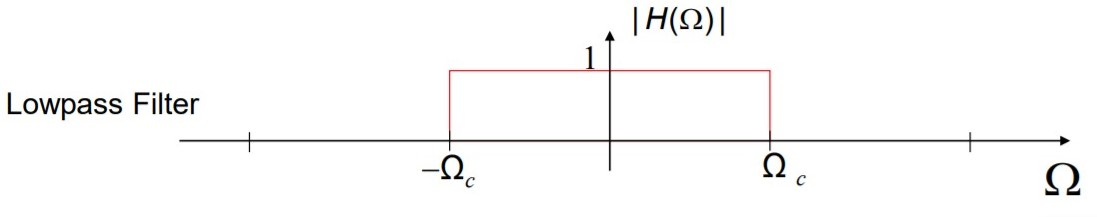
\includegraphics[width=9cm]{filter-low}
		\end{center}
		
		\item the dual behaviour is performed by the \textbf{high-pass filter} that allows to pass through the system only frequencies above a value $\Omega_c$;
		\begin{center}
			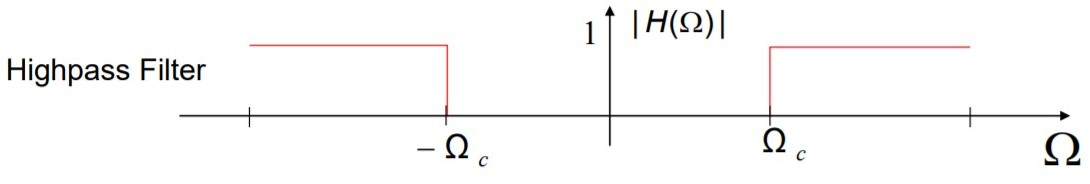
\includegraphics[width=9cm]{filter-high}
		\end{center}
		
		\item \textbf{band-pass filters} are useful to select only a band of frequencies and so allowing only a range $[\Omega_a,\Omega_b]$ of frequencies to be transmitted.
		\begin{center}
			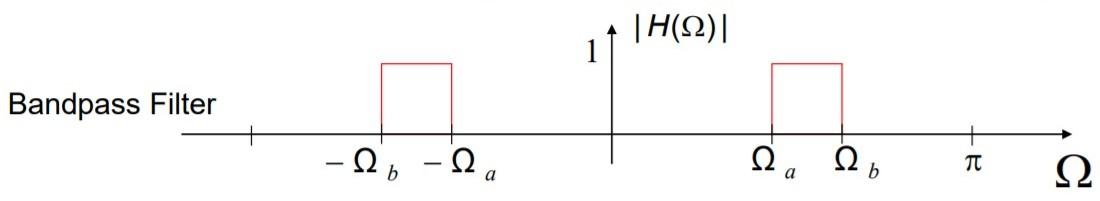
\includegraphics[width=9cm]{filter-band}
		\end{center}
		
		The dual case is the \textbf{stop-band filter} that blocks the frequencies in the specified range.
	\end{itemize}
	All this filters are ideal because in  the real world is impossible to implement this kind of response, but only can approximate them and this is due to the causality of the systems (to implement ideal system we need to know also the future behaviour of the signal).
	
\section{Ideal continuous - discrete conversion}
	The \de{analog to digital conversion} ADC process implies the \de{sampling} (of period $T_s$) of a continuous time signal $x_c(t)$ in order to convert it in a discrete time sequence $x(n)$ (that still an analog signal, it's just a discretization on the time axes of the original signal). In the ideal case the output sequence $x(n)$ can be rewritten as
	\begin{equation}
		x(n) =x_c\big(nT_s\big) = x_c(t) \infsum \delta\big(t-nT_s\big)  
	\end{equation}
	Considering that $\delta\big(t-nT_s\big)$ is a periodic function we can use the Fourier series (with the complex notation) and so
	\begin{align*}
		x(n) & = x_c(t) \infsum c_n e^{j\frac{2\pi}{T_s}nt} \qquad \leftarrow c_n = \frac 1 {T_s} \four{\delta(t)}\Big|_{n} = \frac 1 {T_s} \\
		&= \frac{x_c(t)}{T_s} \infsum e^{j\frac{2\pi}{T_s}nt}
	\end{align*}
	Let's consider now to apply the Fourier transform on this signal substituting $n = -k$ we can determine that
	\begin{equation}
		\four{x_c(nT_s)} = X_c(\Omega) * \frac 1 {T_s}\sum_{k=-\infty}^\infty \delta\left(\Omega- \frac{2\pi}{T_s}k\right) = \frac{1}{T_s} \sum_{k=\infty}^\infty X_c\left(\Omega - \frac{2\pi}{T_s}n \right)
	\end{equation}
	This represent the ideal definition of the frequency spectrum of a sampled signal. In particular we can note that the spectrum of the signal is the exact infinite replica of the continuous spectrum $X_c(\Omega)$ with the spectral replicas distances by a value $\frac{2\pi}{T_s}$, as shown in figure  \ref{fig:conv:replicas}.
	
	\begin{figure}[bht]
		\centering
		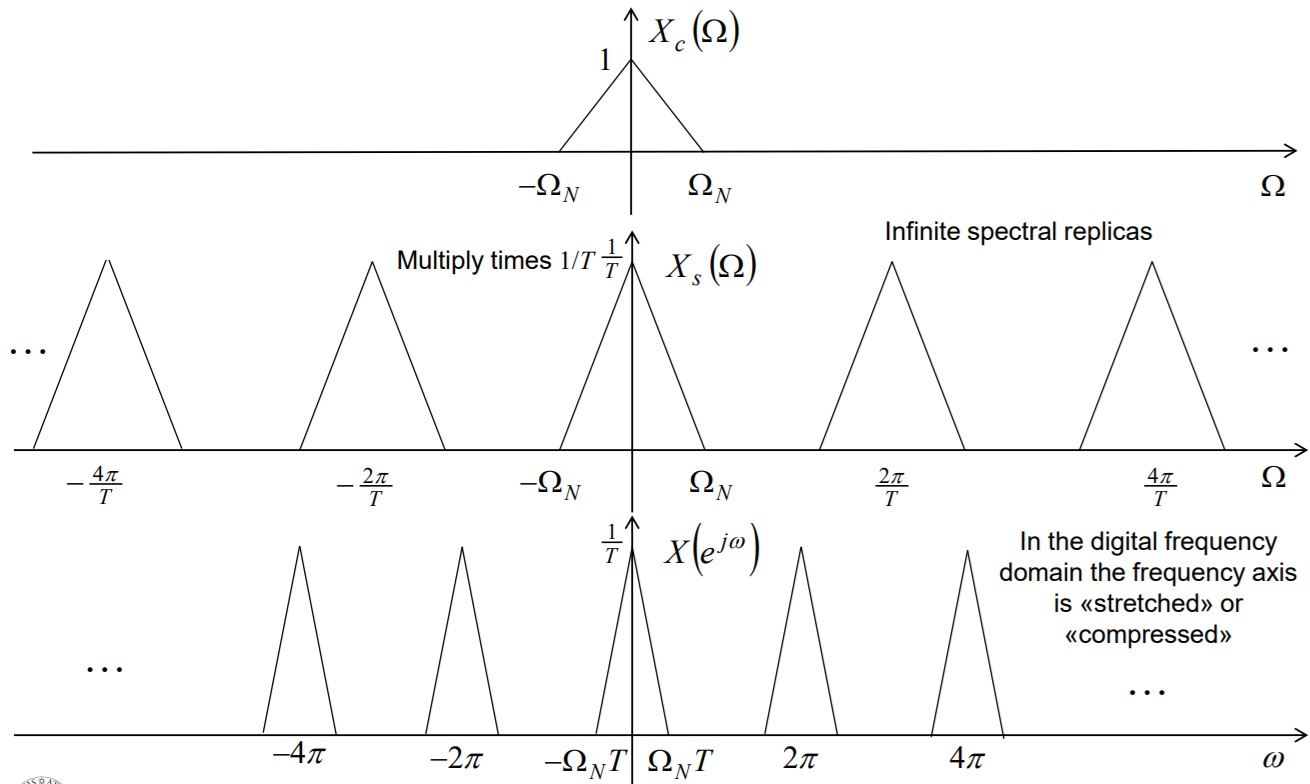
\includegraphics[width=\linewidth]{replicas}
		\caption{from above: frequency spectrum $X_c(\Omega)$ of the signal $x_c(t)$, frequency spectrum of the sampled signal $x(nT_s)$ for the continuous time Fourier transform and then the spectrum $X(e^{j\omega})$ considering the discrete time Fourier transform.} 
		\label{fig:conv:replicas}
	\end{figure}
		
	Considering $x(nT_s)$ as a discrete time signal $x(n)$ we have a re-scalation of the time axes and determine an identical spectrum that doesn't depend on the sampling period $T_s$. Considering that $\Omega T = \omega [rad]$ we have a relation that's independent from the time and so is more a \textit{digital} definition. We can so use the discrete Fourier transform
	\[ x(n) \quad \mapsto \quad X(e^{j\omega})\]
	and by representing the spectrum (figure \ref{fig:conv:replicas}) the replicas are now at multiples of $2\pi$ (having rescaled the axes of a factor $T_s$).
	
	\subsection{Nyquist sampling theorem}
		The \de{aliasing} problem arise when the spectral replicas of the signals (due to the sampling) tends to overlap and happens when the sampling period is to high (or the sampling frequency is too low in respect to the frequencies of the signal). When this happens that we lose too much information from the original signal and so it's impossible to reconstruct it in an acceptable manner. 
		
		\begin{example}{: sampling of a sine wave}
			Let's consider a sine wave of period $T_0$, if we consider a sampling period $T \ll T_0$ than we can observe that having a lot of samples allows us to \textit{decompose} with good approximation the original sine wave, while considering a sampling period $T \backsim T_0$ than most of the information are lost and the constructed signal isn't good enough.
		\end{example}
		
		The aliasing problem must always be avoided because the loss of information is irrecoverable and in order to do so we have to decrease the sampling period $T_s$ (increasing the sampling frequency $f_s$) in order to avoid the overlap of replicas. Given the maximum frequency $\Omega_n$ of the spectrum of the signal in order to avoid aliasing we have to make sure that
		\[ \Omega_n < \frac \pi {T_s} \]
		This represent the base of the \de{Nyquist Shennon sampling theorem}: determining in fact the frequency $f_n = \Omega_n/2\pi$ we can state that
		\begin{equation}
			2\pi f_n < \pi t_s \qquad \Rightarrow \quad f_n < \frac{f_s}{2} \quad \leftrightarrow \quad \omega_n < \pi
		\end{equation}
		and so the signal frequency should always be less then half of the sampling frequency. In particular we refer to $f_s/2$ as the \de{Nyquist frequency} and determines the maximum allowable frequency of the input signal in order to not have aliasing.
		
	\subsection{Sample \& hold}
		To implement a real analog-digital converter we have to consider the continuous-discrete time converter that's preceded by an \de{anti aliasing filter} $H_a(\Omega)$, a low-pass filter that stops frequencies above the Nyquist one in order to avoid (or at least reduce) the aliasing problem.
		
		Consequently to the sampler we need to have a \de{ZOH} Zero Order Hold filter that allows to put a constant output and refresh the out (setting it equals to the input) every sampling period $T_s$. To complete the description of the analog-digital conversion we also need a quantizer block (to discretize the analog function in the values range) and an encoding block that determines a digital output. 
		
		\begin{figure}[bht]
			\centering
			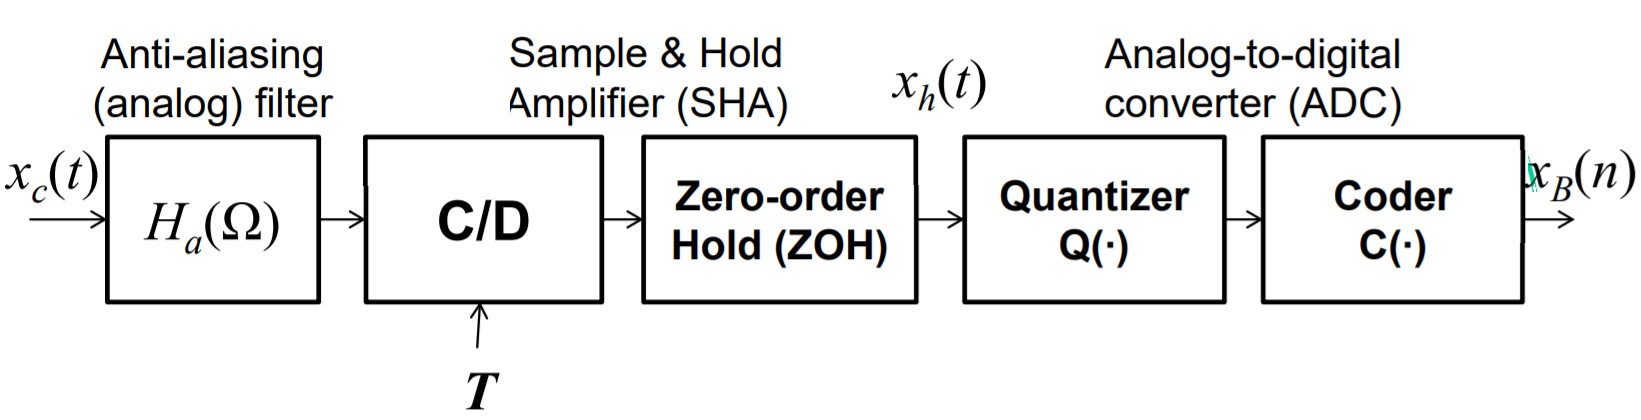
\includegraphics[width=10cm]{adc-steps}
			\caption{composing block of a analog digital converter unit.}
		\end{figure}
	
		
	
	
	
	
	
	
	
	
	
	\chapter{Discrete and fast Fourier transform}
\section{Discrete Fourier transform}
	The \de{Discrete Fourier Transform} (DFT) is different from the previously discussed Discrete Time Fourier Transform (DTFT); in this second case in fact the variable $\omega$, expressed in radians, is real evaluated, while in the discrete Fourier transform. Working instead with the \dft we compute a transform for a finite number of frequency samples $\omega_k \ [rad]$ with $k=0,\dots, N-1$: with this definition we can consider the DFT as a sampling of the transform in the frequency domain. In this case the discrete transform can be computed as
	\begin{equation} \label{eq:ft:dft}
		X(k) = \sum_{n=0}^{N-1} x(n) e^{-j \frac{2\pi}{N}kn} \sum_{n=0}^{N-1} x(n) W_N^{kn} \qquad \forall \ k = 0,1,\dots, N-1
	\end{equation}
	where the term $W_n^{kn}$ is referred as the \textbf{twiddle factor}.
	
	In a practical way the \dft is a sampling of the zeta transform of $N$ samples $\omega_k$ equispaced on the complex unit circle of the $\mathscr Z$ transform of the signal. Increasing the number of $N$ we decrease the \textit{distance} of $\omega_k$ and for $N\rightarrow\infty$ the DFT converges to the discrete-time Fourier transform.
	
	The \dft is not an approximated version of the DTFT, in fact for the same frequency $\omega_k$ the values are the same, but it's only a pure sampling of the continuous transform. \vspace{3mm}
	
	The \dft, in this sense, allow to estimate automatically (that can in fact be computed by machines) the transform of generic non deterministic signals. In practise we don't use the \dft but the \de{Fast Fourier Transform}, a class of complementary algorithms that allows to compute the transform in a faster way (respect to the DFT definition). \vspace{3mm}
	
	Considering the equation \ref{eq:ft:dft} we can see that this expression maxes sense only for signal with a finite number of sample (points); in particular to correctly compute the \dft the number of samples for the sequence $x(n)$ is truncated to $N$ (and having less samples than the decided resolution for $N$, we have to decrease the number of sampling in the transform). The number of frequency samples has to be equal or greater to the number of signal samples.
	
	\paragraph{Inverse Discrete Fourier Transform} In order to compute instead the \de{Inverse Discrete Fourier Transform} (IDFT) we can use the following definition:
	\begin{equation} \label{eq:ft:idft}
		x(n) = \frac 1 N \sum_{k=0}^{N-1} X(k) e^{j\frac{2\pi}{N} kn} \qquad \forall \ n = 0,1,\dots,N-1
	\end{equation}
	This is indeed the inversion of the linear problem of the equation \ref{eq:ft:dft} considering that there are $N$ equations ($X(i)$ for $i=0,\dots, N-1$) having $N$ samples each. Considering that the coefficients are $W_N^{kn}$ we can define the vectorial form of equation \ref{eq:ft:dft} as $\boldsymbol X = W \boldsymbol x$ and so $\boldsymbol x = W^{-1} \boldsymbol X$ (where $K \in \mathds R^{N\times N}$ is the coefficient matrix that's for sure non singular).
	
\subsection{Time aliasing problem}
	Given an arbitrary sequence $x(n)$ whose discrete time Fourier transform is expressed as $X(e^{j\omega})$. By computing the inverse discrete time Fourier transform we can simply reconstruct the original signal, however if we consider the \dft  $X(k)$ of the signal and we invert the result we see that the reconstructed signal $\tilde x(n)$ that's equal to the original signal only for a finite number of samples, and in particular $\tilde x(n) = x(n)$ only for $n=0,1,\dots, N-1$ and only if $N$ is longer then the input sequence length.
	
	Applying the definition of inverse \dft (eq. \ref{eq:ft:idft}) we can see that the reconstructed signal $\tilde x(n)$ must be necessarily a periodic function in time (due  to the linear combination of the twiddle factors) and so
	\[ \tilde x(n) = \frac 1 N \sum_{k=0}^{N-1} X(k) e^{j\frac{2\pi}{N} kn} = \sum_{r=-\infty}^\infty x(n-rN) \]
	
	Given $L$ the number of non-zero samples of the original signal $x(n)$ and compute a \dft with $N$ samples; if $N<L$ then we have the time aliasing problem, while we don't see this problem for $N\geq L$. The number of overlapping samples is equal to $L-N$. If we want only to perform a spectrum analyses (that wont' be followed by a reconstruction) this relations are not necessary (and we can choose any value of $N$).
	
	\begin{SCfigure}[2][bht]
		\centering 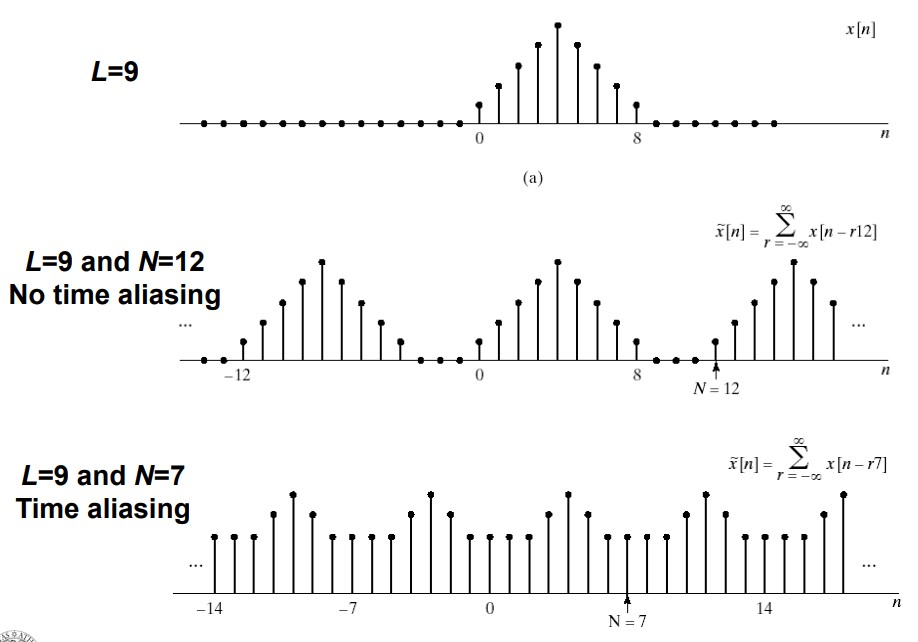
\includegraphics[width=8.5cm]{time-aliasing}
		\caption{original sequence $x(n)$ (on top) with $L=9$ and reconstructed signals $\tilde x(n)$ changing $N$ to $12 (>L)$ and $7 (<L)$. }
	\end{SCfigure}
	
	This concept is the dual result of the spectral replicas that are present in the sampling process on the time domain (in this case we are sampling in the frequency domain and so we have aliasing replicas in time domain).

\subsection{Properties}
	The \dft is a \textbf{linear operator}, in fact given two sequences $x_1(n),x_2(n)$ having discrete transforms $X_1(k),X_2(k)$ then
	\[ a x_1(n) + b x_2(n) \quad \mapsto \quad a X_1(k) + bX_2(k) \qquad \forall a,b \in \mathds R \]
	In particular if the two sequences have different length (for example $N_1 < N_2$) a number of $|N_2-N_1|$ should be added to the shorter sequence, so by doing a \textbf{zero padding}.
	
	We can also consider the \textbf{circular shifting} property that given a sequence $x(n)$ of $N$ samples with \dft $X(k)$, then given a time shift of $m\in \mathds Z$ samples in time determines a sequence
	\[ \tilde x(n-m) \ n = 0,\dots, N-1\quad \mapsto \quad X(k) e^{-j \frac{2\pi k}{N}m} \]
	where $\tilde x(n)$ is the \textit{infinite repetition} of the signal $x(n)$ (concatenation of the same signal). If the original signal $x(n)$ is real evaluated, then $\Re \{ X(k) \} = \Re \{ X(N-k) \}$ (even symmetry on the real axis) and $\Im \{X(k)\} = - \Im \{X(N-k)\}$. 

	Another property is the \textbf{circular convolution} and so given two signals $x_1,x_2 \mapsto X_1,X_2$, then
	\begin{equation}
		x_3(n):=x_1(n) * x_2(n) \mapsto X_1(k)X_2(k)  = X_3(k) \qquad k = 0,\dots, N-1
	\end{equation}
	By computing now the inverse \dft (with $N$ samples) on this result the result that we get is not the original signal $x_3(n)$, but $\tilde x_3(n)$ that's equal to $\tilde x_1(n) * x_2(n) = x_1(n) * \tilde x_2(n)$ (and this is due to the periodicity of the signals). Considering that this convolution is performed over $N$ samples, this operation is now called \textbf{circular convolution} $x_1(n) \circconv{N} x_2(n)$ defined as
	\begin{equation}
		x_1(n) \circconv{N} x_2(n) : = \sum_{m=0}^{N-1} x_1(m) \tilde x_2(n-m)
	\end{equation}
	Considering that $x_1$ consists of $L$ values, while $x_2$ consist of $P$ point, than if the \dft sampling point is equal to $N \geq L + P - 1$ then $x_1(n) * x_2(n) = x_1(n) \circconv N x_2(n)$, otherwise the result of the linear convolution and the circular one can be different.
	
	\paragraph{Impulse response} As described at page \pageref{sec:impulseresponse}, we denote as $h(n)$ the impulse response of a system and in case of a finite impulse response (FIR) one we have that $h(n) \neq 0$ for $n=0,\dots,P-1$. Assuming to have an input sequence $x(n)$ fed into the system will determine an output sequence $y(n)$ that's equal to
	\[ y(n) = x(n) * h(n) \] 
	
	Considering that also the input $x(n)$ as a finite number $L$ of samples, then the length of the convolution $y(n)$ will be different from zero for $n=0,\dots, L+P-2$ (and so it present $L+P-1$ samples). In general a way to solve this kind of problem can be solved in the frequency domain. Considering the discrete time Fourier (DTFT) transform $\F$, known the transforms $H(e^{j\omega}), X(e^{j\omega})$ of the system impulse response and input sequence, than the output can be computed as
	\[ Y(e^{j\omega}) = H(e^{j\omega}) X(e^{j\omega}) \qquad \xrightarrow{\mathscr{F}^{-1}} \quad y(n) \]
	In general this operation using the \dft (DFT), that's practically what happens, is more complex. Given the two discrete transform $X(k),H(k)$ of both the input and the impulse response, we can compute the output frequency response $Y(k) = H(k) X(k)$ that can be inverted to $y(n)$. In order to do perform this operation correctly (and not losing information due to time aliasing) the two transform have to be computed doing a zero padding for $x(n)$ with $P-1$ zero and a padding of $L-1$ zero for $h(n)$: in this case we are sure that the product $X(n)H(n)$ has a number of samples $N = L+P$ that's greater than the $L+P-1$ due to the convolution.

\section{Fast Fourier transform}
	The \de{\fft}, as already stated, is not the same as the \dft but represent a class of algorithms that are implemented to compute the Fourier transform in a \textit{faster} way (by doing less mathematical computation than the original statement).
	
	Starting from the definition on page \pageref{eq:ft:dft} of the \dft we can see that to determine the spectrum we need to perform $N-1$ complex addition and $N$ complex multiplications for each spectral sample, and so the full number of operation to perform is
	\[ N(N-1) \textrm{ complex addition} \quad + \quad N^2 \textrm{ complex multiplication} \]
	Considering that computers can't handle complex number but only real values, it means that one complex multiplication corresponds to 4 multiplications and 2 additions in the real domain (and one complex addition corresponds to 2 real additions). We can see that in general the order of complexity of the \dft is equal to
	\[ \mathcal O \big(N^2\big)\]
	
	The \fft allow to reduce the order of complexity of the operation op to the value $\mathcal O \big(N \log_2 N\big)$ (that's the ideal target value for all the algorithms) then $N$ is a power of 2, and so can be rewritten as $N = 2^\nu$ with $\nu \in \mathds N$. When this conditions is not met, usually the input sampled signal is subdivided in sequences that met the condition, perform the FFT and then recombine the result.
	
\subsection{Decimation in time FFT}
	The basic idea of the \de{decimation in time} DIT \fft algorithm is to recursively decompose the original DFT into more transforms with smaller number of points obtained through bisection.
	
	Considering for example the sequence $x(n) \neq 0$ for $n=0,\dots, N_1$ with $N = 2^\nu$, we can compute two subsequence determined by the sample in even $x_e$ and odd $x_o$ positions, having $N/2$ samples each:
	\[ \underbrace{x(0),x(2),\dots,x(N-2)}_{x_e(n) = x(2r)} \qquad \underbrace{x(1), x(3),\dots, x(N-1)}_{x_o(n) = x(2r + 1)}  \]
	
	Based on the definition (eq. \ref{eq:ft:dft}) of the \dft, we can compute the transform as
	\[ X(k) = \sum_{n=0}^{N-1} x(n) W_N^{kn} = \sum_{r=0}^{\frac N 2 - 1 } x(2r) W_N^{2rk} + \sum_{r=0}^{\frac N 2 - 1} x(2r+1) W_N^{(2r+1)k} \]
	where $W_N = e^{-j\frac{2\pi}{N}}$ is the twiddle factor. We can see that $W_N^2 = W_{N/2}$, in fact
	\[ W_N^2 = e^{-j\frac{2\pi}{N} 2 } = e^{-j\frac{2\pi}{N/2} } = W_{N/2} \]
	and so the previous expression can be rewritten as
	\[ \begin{aligned}
		X(k) & =  \sum_{r=0}^{\frac N 2 - 1 } x_e(r) W_{N/2}^{rk} + W_{N}^k  \sum_{r=0}^{\frac N 2 - 1 } x_o(r) W_{N/2}^{rk} \\ & = X_e(n) + W_N^k X_o(k)  
	\end{aligned} \qquad \qquad \qquad k = 0,\dots,N-1\]
	We can now see that the first sum corresponds to the \dft of the original signal computed only on the even position of $x(t)$, while the second sum corresponds to the odd elements. We can see that computing the transforms $X_e(k),X_o(k)$ requires a number of operation proportional to $(N/2)^2 = N^2/4$, requiring so $1/4$ of the original operations to perform the \textit{pure} transform $X(k)$. If we neglect the time computation of performing the addiction of $X_e+X_o$, than the overall number of operation is
	\[ X_e(k) + X_o(k) \propto \frac{N^2}{4} + \frac{N^2}{4} + N = \frac{N^2}{2} + N \leq N^2 \]
	where the last inequality is always verified for $N>2$.
	\begin{SCfigure}[2][bht]
		\centering 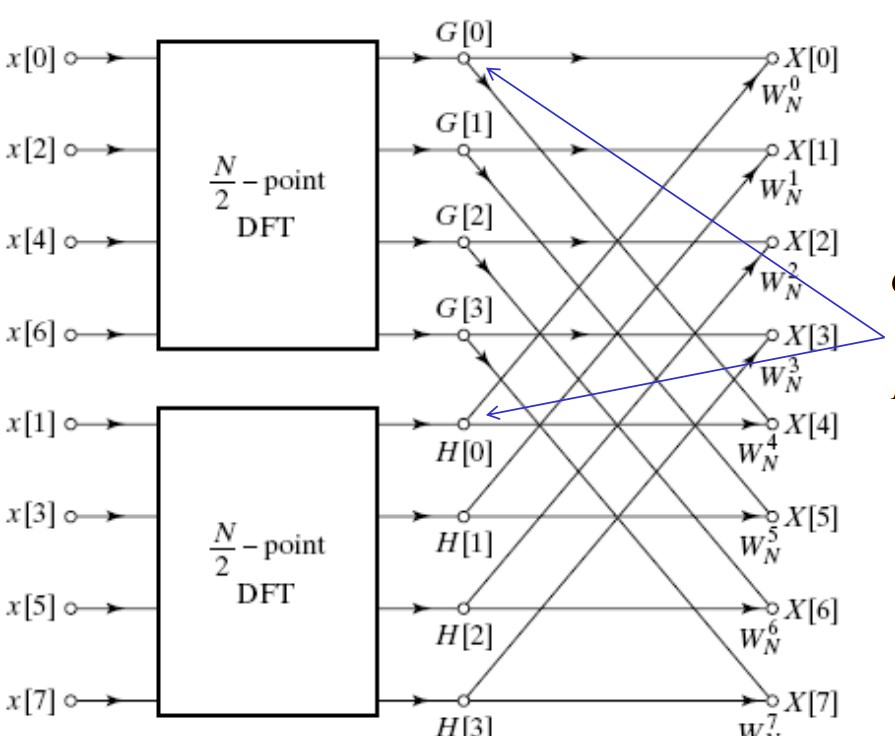
\includegraphics[width=6cm]{fft-dec-graph}
		\caption{graph representing the computation that are needed to be performed to compute the fast Fourier transform using the decimation in time algorithm for $N=8$ samples.}
	\end{SCfigure}
	
	
	By applying recursively this concept for sequences until we reach input signals of 2 samples each, the overall computational complexity of the \dft  drops from $\mathcal O(N^2)$ to $\mathcal O(N\log_2N)$.
	\begin{SCfigure}[2][bht]
		\centering 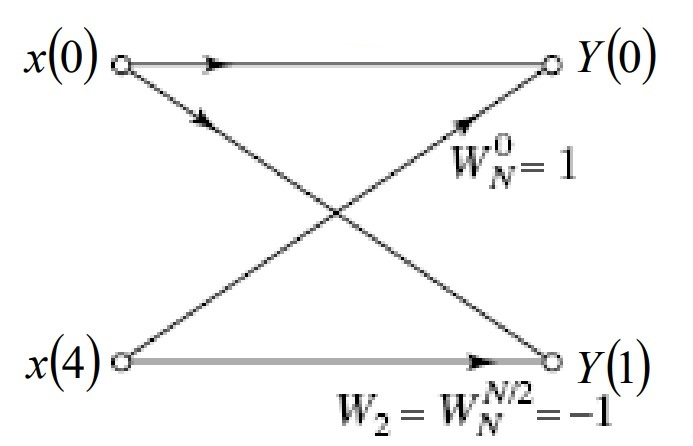
\includegraphics[width=4cm]{fft-dec-graph-bin}
		\caption{graph representation of the \fft using the decimation in time algorithm computed on 2 points.} \label{fig:dft:ditsing}
	\end{SCfigure}
	
	In the single stage (figure \ref{fig:dft:ditsing}) the transform become just a summation of the points we are considering, in fact
	\[ Y(0) = x(0) + x(1) \qquad \qquad \qquad Y(1) = x(0)-x(1) \]	
	Given the initial number $N$ of samples, then it means that we have to compute $2$ operation for each of the $N/2$ \textit{basic block} for the Fourier transform, and so the complexity presents a linear order. Laterly we need to \textit{join} the singularly computed block considering that the different twiddle factors are going each time to shift in the complex axis the spectrum inherited from the previous block; each stage also presents a linear order of complexity. The number of stages to be computed is equal to $\nu = \log_2N$ and so that's why the overall complexity of the algorithm is
	\[ \mathcal O\big(N\log_2 N \big) \]
	
	
	\begin{SCfigure}[2][bht]
		\centering 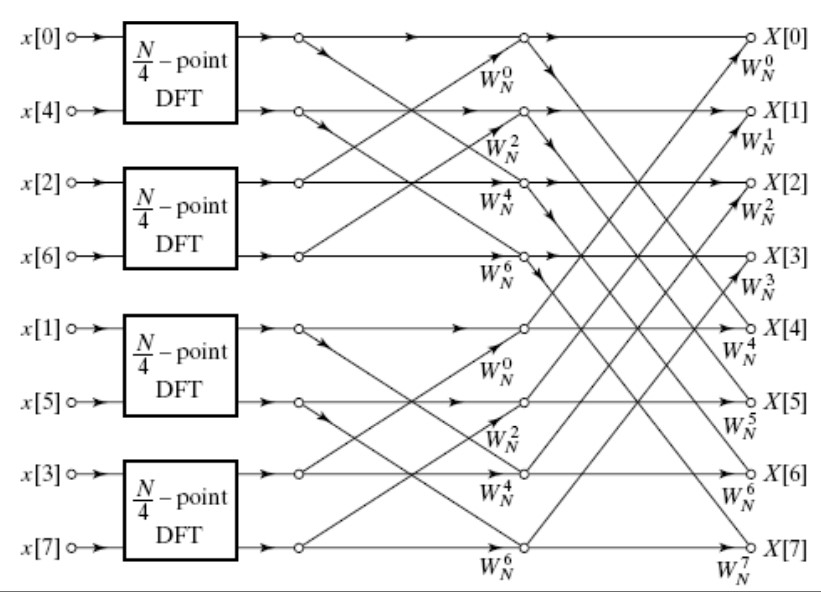
\includegraphics[width=7cm]{fft-dec-graph-comp}
		\caption{complete graph representing the computation to do with the decimation in time algorithm for $N=8$ samples. The transform of 2 value is shown in figure \ref{fig:dft:ditsing}.}
	\end{SCfigure}
	
	\paragraph{Modularity of the FFT algorithm} A point of force of this algorithm is it's recursion and modularity that allows to easily compute and \textit{see} different stages and tasks due to the \textit{butterfly structure}. Another strong point of implementation is that each operation permits to overwrite the spectrum on the same memory cell of the original signal. Also twiddle factors that need to be computed are equal for butterflies at each stage, and so they have to be computed one.
	
	In general the butterfly can be represented as in figure \ref{fig:dft:decstage} where the only thing that changes are the indexes $p,q$; to reduce the computation we can also see that 
	\[ W_N^{r + \frac{N}{2}} = W_N^r W_N^{\frac N 2}  = - W_N^r \]
	where $r$ depends on the stage we are considering.
	
	\begin{figure}[bht]
		\centering 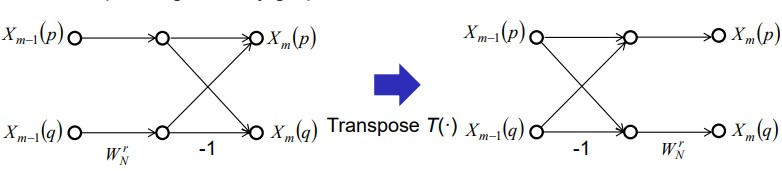
\includegraphics[width = 8cm]{fft-dec-stage}
		\caption{schematic representation of a generic stage of the decimation in frequency FFT algorithm.}
		\label{fig:dft:decstage}
	\end{figure}
	
	Another computational aspect that we might see is the use of memory; in fact samples are stored not in order for computation, however we can see that that the bits are inserted in \textbf{binary flip revered order} as in the example on table \ref{tab:dft:reversed}.
	\begin{SCtable}[2][bht]
		\centering
		\begin{tabular}{c c | c c}
			$x(0)$ & 000 & 000 & $X(0)$ \\
			$x(4)$ & 100 & 001 & $X(1)$ \\
			$x(2)$ & 010 & 010 & $X(2)$ \\
			$x(6)$ & 110 & 011 & $X(3)$ \\
			$x(1)$ & 001 & 100 & $X(4)$ \\
			$x(5)$ & 101 & 101 & $X(5)$ \\
			$x(3)$ & 011 & 110 & $X(6)$ \\
			$x(7)$ & 111 & 111 & $X(7)$ \\
		\end{tabular} \caption{example of binary revered order that's used in performing the the fast Fourier transform.} \label{tab:dft:reversed}
	\end{SCtable}
	
\subsection{Decimation in frequency FFT}
	This kind of FFT algorithm is an alternative to decimation in time one and in general it's complementary and it's based on the partition of the original signal in sub samples and so starting from the transform $X(k)$ we determine the partition in even and odd partition in the frequency:
	\[ X(k) \qquad \rightarrow \quad X_e(k ) = X(2k) \quad X_o(k) = X(2k+1) \]
	The concept of work is similar to the decimation in time and the algorithm presents a complexity of $\mathcal O(N\log_2N)$. This operation can be performed considering the \textbf{transpose property of the graph}: given a graph $\delta(N,\varepsilon)$ of $N$ edges and $\varepsilon$ edges, then it's transpose $\delta^t(N,\varepsilon')$ (where we reverse the edge direction, and so also input/output are reversed) the input-output relation of the graphs is the same. 
	
\section{Spectral estimation}
	The \de{spectral estimation} is an analyses of the signal that tends to provide information about the behaviour of the system.
	
	Considering that usually signals are not deterministic (but stochastic), this operation is usually hard to perform and handle; in general this operation is classified (figure \ref{fig:dft:estimation}) depending on the type of signal (deterministic or random) and it's stationarity.
	
	\begin{SCfigure}[1][bht]
		\centering 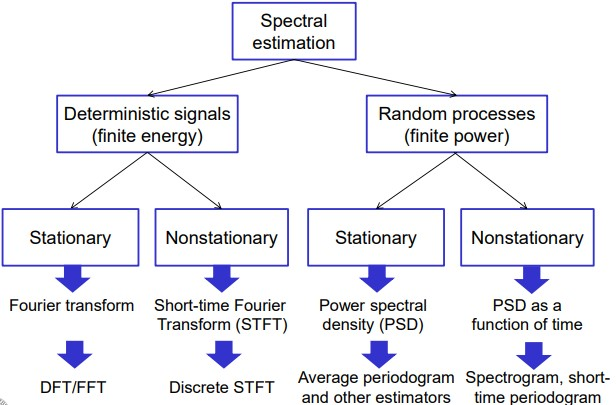
\includegraphics[width=7cm]{spectral-estimation}		
		\caption{classification of the spectral estimation} \label{fig:dft:estimation}
	\end{SCfigure}
	
	If a system is stationary the quality of estimation doesn't depend on the time on which we perform the estimation itself, while this isn't true for non-stationary signals on which we want to track all the changes of the signals.
	
	\paragraph{Deterministic stationary estimation} Focusing on a deterministic stationary signal $x_c(t)$, performing the spectral estimation is in theory easy because (with the Fourier transform) we can compute it's spectrum $X_c(\Omega)$. In practise however we cannot reach this exact value, but we get an approximation $\hat X_c(\Omega) \approx X_c(\Omega)$.
	
	\begin{figure}[bht]
		\centering
		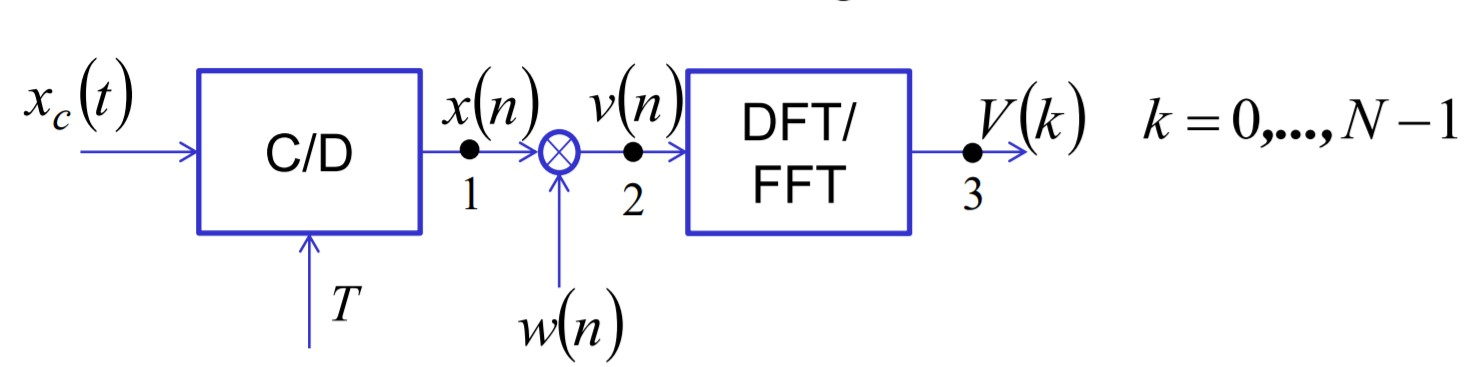
\includegraphics[width=8cm]{deterministic-estimation}
		\caption{step encountered while estimating a deterministic signal.}
		\label{fig:dft:deterministicestim}
	\end{figure}
	
	As we can see in figure \ref{fig:dft:deterministicestim} when dealing with a real world application of spectral estimation, the original signal $x_c(t)$ must be discretized in the time axis with a sampling period $T_s$ (and in this case we can consider an ideal component, but in reality just only this operation can introduce errors due to acquisition noises...); at this point the ideal Fourier transform of the input signal becomes
	\[ X(e^{j\omega}) = \frac 1{T_s} \sum_{k=-\infty}^{\infty} X_c \left( \frac \omega {T_s}+ \frac{2\pi k}{T_s} \right)  \]
	As we can see this discretization introduces to the original spectrum a scaling factor of $1/T_s$ and also introduces the spectral replicas at multiple frequencies of $2\pi/T_s$, and in  this case we neglect the quantization/acquisition noises.
	
	With the signal acquired the numerical tool that we can use to estimate the spectrum are the DFT/FFT algorithms that uses a finite number $N$ of samples (on which to compute the spectrum), and so the sequence $x(n)$ must be \textit{truncated} to such a number of samples: this operation is referred as \textbf{windowing}. This operation can be modelled as a multiplication of the initial sequence $x(n)$ with the function $w(n)$ defined as
	\[ w(n) = \begin{cases}
		1 \qquad& n=0,\dots,L-1 \\ 0 & \textrm{otherwise}
	\end{cases} \]

	At this point we can see that the DFT/FFT algorithm are applied on the sequence $v(n) = x(n)w(n)$ (on which we can see that $v(n) \neq 0$ for $n = 0,\dots, L-1$): by a spectral point of view this means that the estimated spectrum (considering the ideal Fourier transform) becomes
	\[ V(e^{j\omega}) = X(e^{j\omega}) * W(e^{j\omega}) = \frac 1{2\pi} \int_{-\pi}^\pi X(e^{j\theta}) W(e^{j(\omega-\theta)}) \, d\theta \neq X(e^{j\omega}) \]
	As a rule of thumb we see that the number of point $N$ on which we compute the \dft must be greater of equal to $L$, the number of \textit{windowed} samples (in reality $N$ can be less then $L$ if we don't have to go back in the time domain because the time aliasing won't be a problem, but we decrease also the \textit{resolution}).\\
	The final output $\hat X_c(\Omega) = V(k)$ also contains the problem of the spectral sampling.

	\paragraph{Effects of windowing on the spectral estimation of a sine wave} Considering the continuous time sinusoidal signal $x_c(t) = A \cos(\Omega_0t + \theta_0)$, it's spectrum (figure \ref{fig:dft:cosspec}) consists of two dirac pulses at frequencies $\pm\Omega_0$ having complex amplitude $\frac  A2 e^{-j\theta_0}$.
		
	\begin{SCfigure}[2][bht]
		\centering 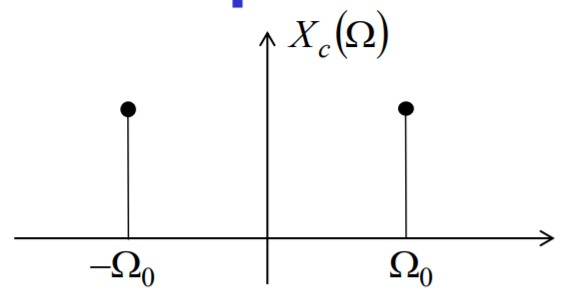
\includegraphics[width=5cm]{sin-spect}
		\caption{magnitude spectrum of the signal $A \cos(\Omega_0t+\theta_0)$.}
		\label{fig:dft:cosspec}
	\end{SCfigure}

	Assuming to sample the signal with a sampling period $T_s$ we determine the sequence $x(n) = A \cos(\omega_0n + \theta_0)$ (where $\omega_0 = \Omega_0 T_s$); considering on top of that the windowing the signal on which we can compute the DFT becomes
	\[ v(n) = x(n)w(n) = A w(n) \cos(\omega_0n+\theta_0) = \frac A 2 w(n) e^{j\theta_0} e^{j\omega_0n} +\frac A 2 w(n) e^{-j\theta_0} e^{-j\omega_0n} \]
	where we used the Euler relation. Applying the theoretical discrete-time Fourier transform we know that $\four{e^{j\omega_0n}} = \delta(\omega-\omega_0)$ and so the spectrum can be computed as
	\[ V\big(e^{j\omega}\big) = \frac A 2 e^{j\theta_0} W\big(e^{j(\omega-\omega_0)}\big) + \frac A 2 e^{-j\theta_0} W\big(e^{j(-\omega+\omega_0)}\big) \]
	At this point to determine the \textit{shape} of the estimated spectrum $V$ it's necessary to understand the distortion of the windows and so it's necessary to compute it's Fourier transform:
	\[ W\big(e^{j\omega}\big) = \sum_{n=-\infty}^{\infty} w(n) e^{-j\omega n} =  \sum_{n=0}^{L-1} e^{ -j\omega n} = \frac{1 - e^{-j\omega L}}{1-e^{-j\omega}} = e^{-j\omega \frac{L-1}{2}} \frac{\sin\left(\frac{\omega L}{2} \right)}{\sin \left( \frac \omega 2 \right)} \]
	where the series can be solved considering that $\sum e^{-j\omega n}$ is a geometrical progression. The special function $\sin\left(\frac{\omega L}{2}\right) / \sin\left(\frac \omega 2\right)$ is referred as Dirichlet-Kernel; characteristic of this function is that for $\omega= 0$, the magnitude of the spectrum is equal to $L$ and for each multiple of $2\pi/L$ it's null (figure \ref{fig:dft:dirich}).
	
	\begin{figure}[bht]
		\begin{subfigure}{0.48\linewidth}
			\centering 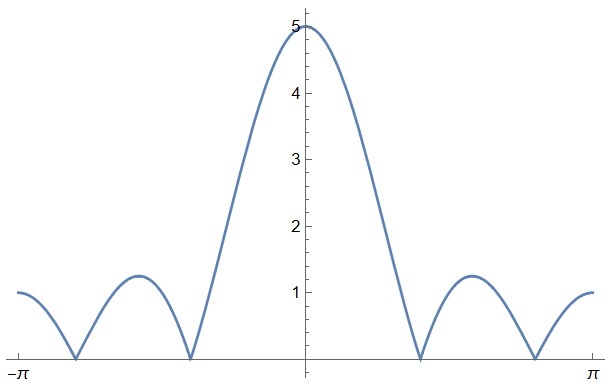
\includegraphics[width=5cm]{dirich-kernel} \caption{}
		\end{subfigure}
		\begin{subfigure}{0.48\linewidth}
			\centering 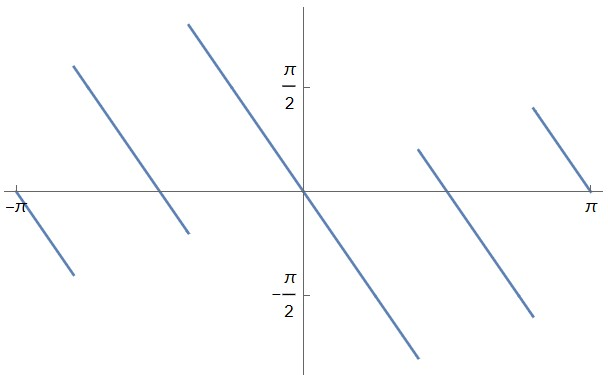
\includegraphics[width=5cm]{dirich-kernel-phase} \caption{}
		\end{subfigure}
		\caption{magnitude (a) and phase (b) of the Dirichlet-Kernel function.}
		\label{fig:dft:dirich}
	\end{figure}
	
	We refer to the \textit{central peek} as the main-lobe (and present a peek value equal to $L$ number of samples used for the windowing), while the other spectral \textit{bell-shapes} are the side-lobes whose maximum values is constantly decreasing for $\omega$ that increase. The parameter $\Delta_w = 4\pi /L$ represent the main-lobe width. The phase of this function is described as \textit{generalized linear phase}. \vspace{3mm}
	
	With that said, in theory the spectrum that we expect from the initial sinusoidal signal $x_c$ are two Dirac pulses, however in reality that spectrum $V(e^{j\omega})$ that we see (after the windowing due to the \textit{truncation} of the signal) is composed by two Dirichlet-Kernel function with main-lobes centred at the frequencies $\omega_0$ on which we expect the Dirac pulses (figure \ref{fig:dft:spectrdistorted}).
	
	\begin{SCfigure}[2][bht]
		\centering 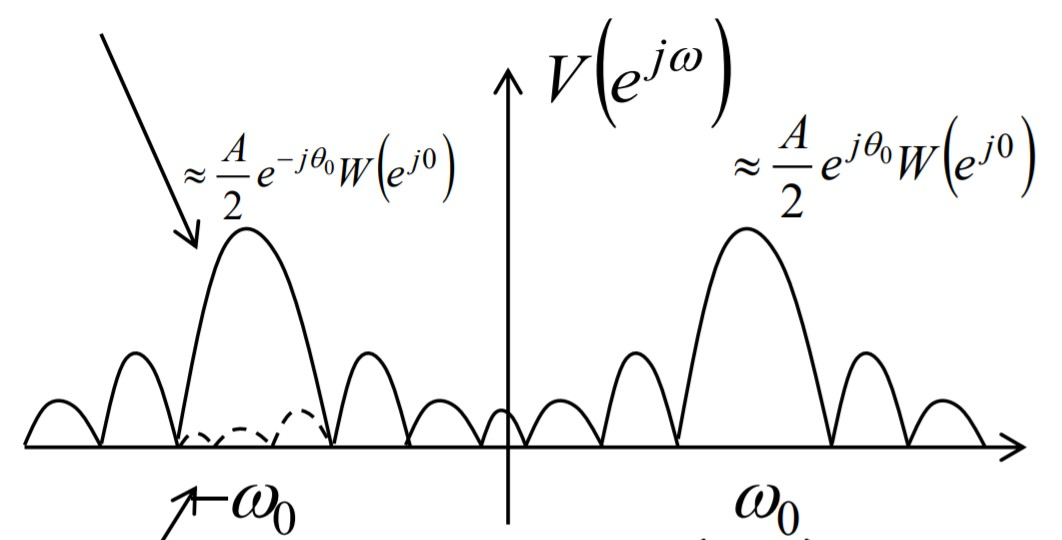
\includegraphics[width=6cm]{sin-modified}
		\caption{spectrum of the signal  $v(n)= x(n)w(n)$ that's distorted due to the windowing.}
		\label{fig:dft:spectrdistorted}
	\end{SCfigure}
	
	To decrease the main-lobe width $\Delta_w$ it's necessary to increase the number of sample $L$ considered on the window $w$ (in fact with $L\rightarrow \infty$ the Dirichlet-Kernel function tends to the Dirac pulse). In real world application we cannot get rid of the lobes of the Dirichlet-Kernel function (we cannot compute the DFT on sequence of infinite samples) and so the associated problems are 
	\begin{itemize}
		\item the \textbf{spectral leakage}: in theory the energy of the original sinusoidal signal is concentrated on the frequencies $\pm \omega_0$, however with the windowing  there's a sort of \textit{leak} that spread the energy over all the frequency axis;
		
		\item the \textbf{spectral infiltration} (related to the leakage) refers to the fact that the side-lobes of a Dirichlet-Kernel might interfere to the main-lobe of the other function (and vice-versa); it can be shown in fact that the ratio between the main-lobe and it's adjacent side-lobe is constant and weakly depend on the number of samples $L$;
		
		\item the \textbf{finite spectral resolution}: considering a signal $x_c(t) = A_1 \sin(\Omega_1t + \theta_1) + A_2 \sin(\Omega_2t + \theta_2)$, the ideal spectrum of the signal consist in Dirac pulses centred at frequencies $\pm \omega_1,\pm \omega_2$, however the estimated spectrum is in the form
		\[ V\big(e^{j\omega}\big) = \sum_i \frac{A_i}2 e^{\pm j\theta_i} W\Big( e^{j(\omega \mp \omega_i)} \Big) \]
		We can see that if the frequencies $\omega_1$ and $\omega_2$ are close together (mathematically $|\omega_1-\omega_2$ is \textit{small enough}) the main-lobes interferes and so the problem of the spectral leakage becomes very important and heavily changes the estimated spectrum. If the frequencies $\omega_1,\omega_2$ are \textit{far apart} this kind of problem might be neglected (figure \ref{fig:dft:spectralresolution}). Increasing the number $L$ the main-lobe width decrease and so we can qualitatively improve the spectral resolution. In order to not distinguish the two peeks (considering $A_1 = A_2$), as a qualitative definition, we must require that
		\[ |\omega_1-\omega_2| > \frac{\Delta_w}{2} \]
				
	\end{itemize}

	\begin{SCfigure}[2][bht]
		\centering 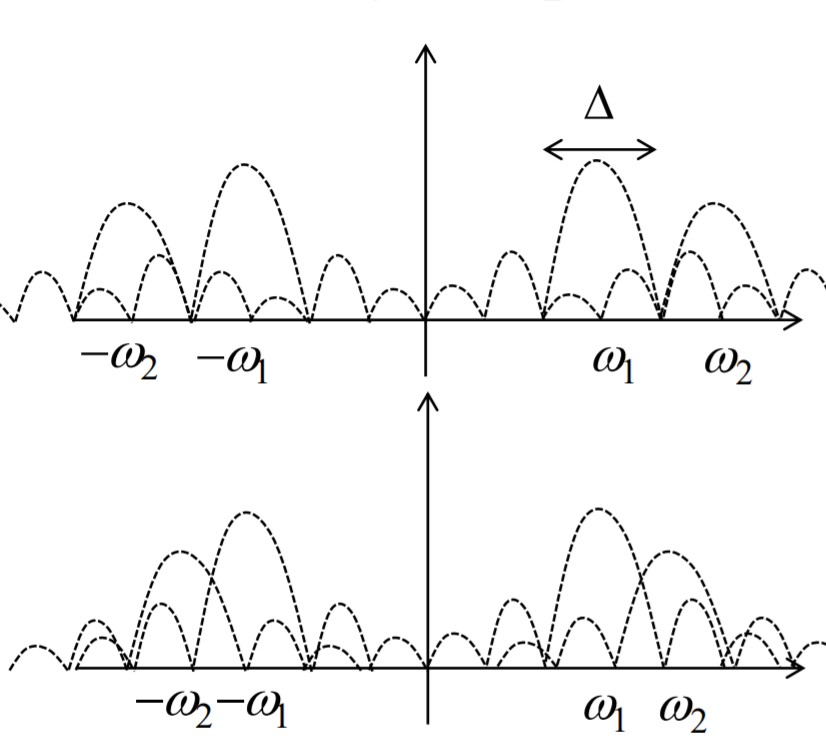
\includegraphics[width=6cm]{spectral-resolution}
		\caption{estimated spectrum of a signal $ A_1 \sin(\Omega_1t + \theta_1) + A_2 \sin(\Omega_2t + \theta_2)$ where the difference $\omega_1-\omega_2$ is negligible (upper) or not (lower) considering the problem of the spectral resolution.} \label{fig:dft:spectralresolution}
	\end{SCfigure}

	In general other window function $w(n)$ have been constructed in order to minimize the errors/problems associated to the spectral estimation (increasing the ratio between the main-lobe and the side-lobes and also decreasing the width $\delta_w$ given the same amount of samples $L$); this is achieved by not having rectangular shape but using smoother functions (table \ref{tab:dft:windowfunctions}, figure \ref{fig:dft:windowfunctions}).
	
	\begin{table} \centering
	\begin{tabular}{c|c|c}
		Windows & side/main-lobe ratio & main-lobe width $\Delta_w$\\ \hline
		rectangular & $-13db$ & $4\pi/L$ \\
		Bartlett (triangular) & $-25db$ & $8\pi/L$ \\
		Hanning & $-31db$ & $8\pi/L$ \\
		Hamming & $-41db$ & $8\pi/L$ \\
		Blackman & $-57db$ & $12\pi/L$ \\
	\end{tabular}
	\caption{list of possible windows with relative side to main-lobe radio (in decibels) and main-lobe width (depending on number of windowed samples $L$).}
	\label{tab:dft:windowfunctions}
	\end{table}
	\begin{figure}[bht]
		\centering 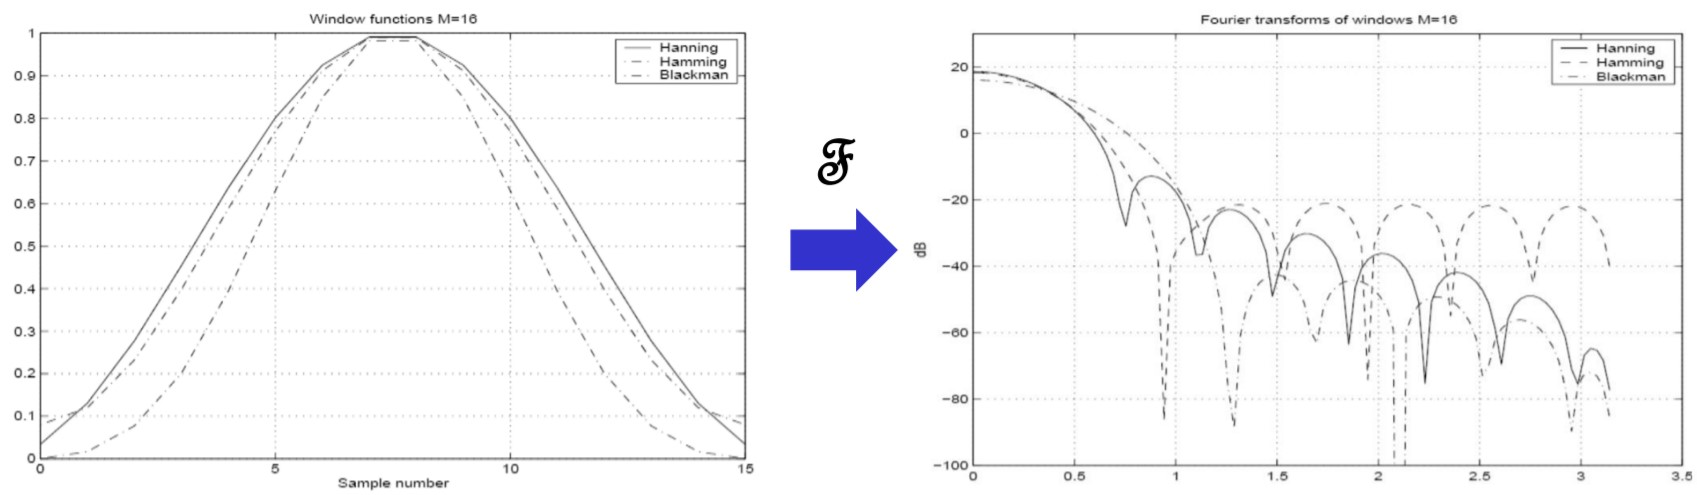
\includegraphics[width=\linewidth]{windowfunctions}
		\caption{windowing functions and relative Fourier transforms.}
		\label{fig:dft:windowfunctions}
	\end{figure}
		
	As we can see window functions with higher side to main-lobe attenuation  present main-lobe width that are higher (impacting so the resolution), but they also reduces the \textit{errors} due to the side-lobes. In particular Hanning, Hamming and Blackman are inside the so called \textbf{cosine class windows} of order $K$ that can generally expressed as
	\[ w(n) = \int_{k=0}^K a_k \cos\left( \frac{2\pi k}{L}n\right) \qquad n = 0,\dots, L-1 \]
	where the coefficients $a_k$ depends on the order $K$ chosen. In particular Hanning ($a_0 = \frac 1 2, a_1 = -\frac 1 2$) and Hamming ($a_0 = 0.54, a_1 = - 0.46$) windows are cosine class windows of order 1, while Blackman has order $2$. As we can see the main-lobe width relates to the order of the function following the relation
	\[ \Delta_w = \frac{4\pi}{L}\big(K+1\big) \]
	
	Fixing the samples $L$ of the transform going the rectangular to the Blackman windows the spectral resolution worsen while the spectral leakage improves (and so it's always a trade-off).	
	
	\paragraph{Frequency discretization} Until now we have computed the continuous spectrum $V(e^{j\omega})$ of the sampled signal, however by computing the \dft (or using \fft algorithms) what we get is just a discretization $V(k)$ (with $k =0,\dots,N-1$) on the frequency domain of the spectrum itself. In particular considering the initial case of the the sinusoidal function $x_c(t) = A \cos(\Omega_0 t + \theta_0)$ changing the number $N$ used for the computation of the DFT might heavily affect the read spectrum, and in particular we can have:
	\begin{itemize}
		\item a \textbf{coherent sampling} happens when one of the spectral samples lies exactly at the frequency $\omega_0$ while the other samples coincides with the zeros due to the window spectrum. In this case the spectrum is clear and the effect of leakage is negligible. This kind of operation can be performed in general only for periodic signals (because it's \textit{easy} to determine the number of samples $N$ that minimize the leakage) due to the fact that the ideal spectrum is composed by a sequence of Dirac pulses;
		\item a \textbf{non-coherent sampling} happens when the peak lies between the two largest spectral samples; in this case we have uncertainty both in the magnitude and in the frequency of the peak. The effect of leakage is evident;
		\item improving the number of samples $N$ on a non-coherent sampling increases the number of spectral samples and so the error in estimating the magnitude and relative frequency of the peak decreases (but the effect of leakage doesn't decrease). 
	\end{itemize}
	
	\begin{figure}[bht]
		\begin{subfigure}{0.32\linewidth}
			\centering 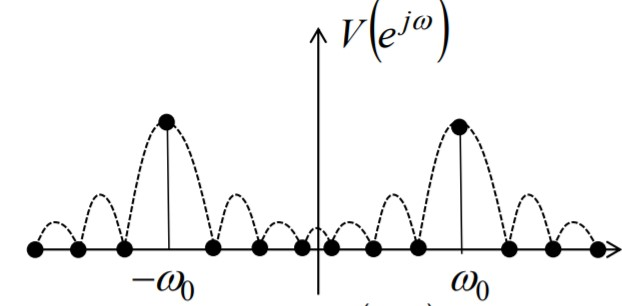
\includegraphics[width=0.9\linewidth]{sampling-1} \caption{}
		\end{subfigure}
		\begin{subfigure}{0.32\linewidth}
			\centering 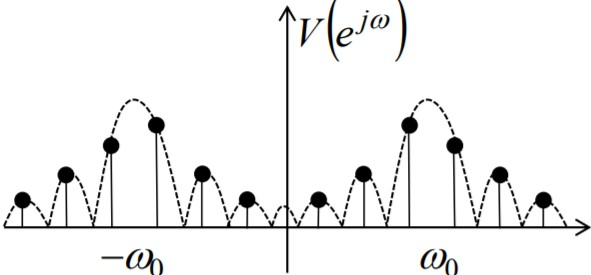
\includegraphics[width=0.9\linewidth]{sampling-2} \caption{}
		\end{subfigure}
		\begin{subfigure}{0.32\linewidth}
			\centering 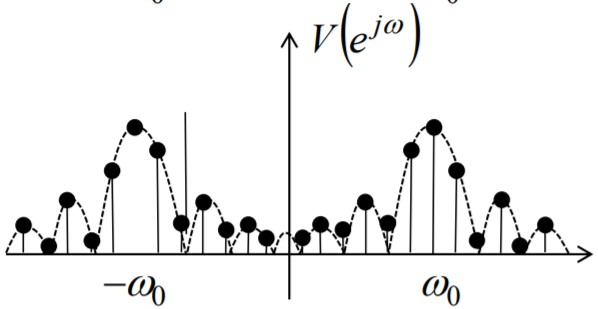
\includegraphics[width=0.9\linewidth]{sampling-3} \caption{}
		\end{subfigure}
		\caption{coherent sampling (a), non-coherent sampling (b) and non-coherent sampling with higher number of samples $N$ (c).}
		\label{fig:dft:samplingvariation}
	\end{figure}
	
	\paragraph{Non stationary deterministic signals} A simple example of non stationary signal is the \textbf{chirp} one defined as a sinusoidal function whose frequency changes linearly over time, and so of the form
	\[ x_c(t) = \cos\big(\Omega(t) t\big)  \qquad \textrm{where } \Omega(t) = \Omega_0t \]
	In this case evaluating the function at the time $t_0$ we expect a DFT having a Dirac pulse centred at frequency $\Omega(t_0)$, while if we evaluate the signal at time $t_1$ we expect a pulse at another frequency $\Omega(t_1)$. In the real world we cannot have this kind of spectrum because we have to compute the transform over a window of the real signal (whose frequency is changing over time); in particular the read spectrum is a sort of \textit{smoothed average} of the peaks in the transform in the range whose samples are extracted. To avoid this problem we can try to reduce the window in time $\Delta t$ (time from the first to last sample) but this impact in the number of samples $L$ recorded (decreasing the frequency resolution). In general
	\begin{align*}
		\textrm{long window} \qquad &\Rightarrow \quad \textrm{high frequency resolution, poor time resolution} \\
		\textrm{short window} \qquad &\Rightarrow \quad \textrm{low frequency resolution, good time resolution}
	\end{align*}
	
	Considering in general that we expect two peaks at frequencies $\Omega_1,\Omega_2$, than the related difference of normalized frequency $\Delta \omega = \Delta \Omega \, T_s$ must be at least equal to half of the main-lobe width, and so in the case of the rectangular window we can see that
	\[ \Delta \omega > \frac{\Delta_w}{2} = \frac{4\pi}{2L} \qquad \Rightarrow \quad \Delta_f \underbrace{L T_s}_{=\Delta t} > 1   \]
	This expression gives the lower bound between time analyses and frequency resolution (where $\Delta_f$ is the frequency difference between the components in the signal).
	
\subsection{Short time Fourier transform}
	The \de{short time Fourier transform}, also known as discrete-time time-varying Fourier transform is a operation that performs DFTs over $L$ samples by \textit{shifting} each time by $R$ samples; ideally we have a \textit{localised} Fourier transforms (and so with a short window we can improve the time resolution) that are spread over all the sample axis. In general we consider $R\leq L$ in order to not lose information (in fact if $R>L$ a number of $R-L$ samples will be lost because they won't be used in the computation of the DFT), while as for the previous cases usually $L\leq N$ in order to have a better read-out of the spectrum.
	
\subsection{Estimation of the power spectral density}
	As seen on page \pageref{eq:prob:psd}, the power spectral density is the Fourier transform of the auto-correlation of a wide sense stationary random process. In real world application it's necessary to estimate this spectrum $\hat \Phi(e^{j\omega})$ that's in general computationally heavier than a single Fourier transform (because the auto-correlation contains a summation in it's definition).
	
	Given a continuous signal $x_c(t)$ sampled with period $T_s$ to determine the sequence $x(n)$ that's then windowed by the window $w(n)$, the estimation of the power spectral density can be achieved in two ways:
	\begin{itemize}
		\item by firstly computing the autocorrelation of the windowed signal that's lately transformed. Starting from the definition of the discrete-time autocorrelation (eq. \ref{eq:four:autocorrelation}, pg. \pageref{eq:four:autocorrelation}) considering as window function the rectangular one with $L$ samples, then the autocorrelation of the sequence $v(n) = x(n)w(n)$ can be computed as
		\begin{equation} \label{eq:dft:windowedauto}
			\hat \phi_v(n) = \frac 1 L \sum_{l=0}^{L-|n|-1} x(l) x(n+l) \qquad \textrm{with } n = 0,\dots,L-1
		\end{equation}
		At this point we can compute the estimation of the power spectral density $\hat \Phi_v(e^{j\omega})$ by computing the Fourier transform $\four{\phi_v(n)}$ of the computed autocorrelation over $L$ samples;
		
		\item by inverting the steps we can firstly compute a discretized sequence of the spectrum $V(k) = \four{v(n)}$ that's then passed through a \textit{power spectral density estimator} that computes $\hat \Phi_v(e^{j\omega})$ (or in practise it's discretization over the frequency axis). This operation is usually peformed by the \textbf{periodogram} that will be described later.
	\end{itemize}
	
	\paragraph{Estimator} An \de{estimator} is any function that, given a random sampled from the population, infers a parameter of the population that's taken from. An example of estimator is the one that, given $M$ person of a cities, tends to compute the average age of the city. The estimator $E\{\cdot\}$ is in this case examples the mean value of the samples that's
	\[ E\{x\} = \frac 1 M \sum_{i=1}^M x_i \]
	where $E\{x\}$ is the estimated age average of the population $x$ and where $x_i$ are the age of the sampled person. \vspace{3mm}
	
	The goal now is to fined a function $g$ that allows to better estimate the power spectral density of a given sequence that's already been transformed (and so it's in the frequency domain). Consider $\boldsymbol x$ as the random vector of all the possible inputs, then the estimated power spectral density $\hat \theta = g(\boldsymbol x)$ becomes a random process that's for each input $\boldsymbol x$, $\theta$ is the realization of the random process.\\
	Consider that $\hat \theta$ is a random process, than it's characterized by a probability density function that can be used to determine the expected value $E\{\hat \theta\}$ and it's variance $\textrm{Var}\{\hat \theta\}$ that, for an ideal estimator, should be $E\{\hat \theta\} = \theta$ and $V\{\hat \theta\} = 0$. In general we defined
	\[ E \{\hat \theta\} = \begin{cases}
		\theta \qquad & \textrm{unbiased estimator} \\
		\theta + c\qquad & \textrm{biased estimator}
	\end{cases}\]
	\[ V\{ \hat \theta \} \xrightarrow{M\rightarrow \infty} \begin{cases}
		=0 \qquad & \textrm{consistent estimator} \\
		\neq 0 & \textrm{inconsistent estimator}
	\end{cases} \]
	In general the problem of the bias of the estimator can be handled, while the same cannot be said for the consistency of the variance. 
	
	\paragraph{Characteristic of the estimation of the autocorrelation} Given the windowed signal $v(n) = x(n) w(n)$, the autocorrelation of each sample can be computed as shown in equation \ref{eq:dft:windowedauto}. Given $X(\cdot)$ the associated random process, the estimation of the random process can be computed as
	\begin{align*}
		E\left\{\hat \Phi_V(n)\right\} & = E \left\{ \frac 1 L  \sum_{l=0}^{L-|n|-1} X(l) X(n+l) \right\} = \frac 1 L \sum_{l=0}^{L-|n|-1} \phi_x(n) \\
		& = \frac{L-|n|}{L} \phi_x(n)
 	\end{align*} 
	This means that this kind of estimation in biased with a variant level depending from the window length $L$ and the \textit{position} $n$ of the sample. In general the performance are good for $n\ll L$. Similarly we can show that this estimation is non consistent, in fact it can be shown that
	\[ V\left\{ \hat \Phi_V \right\} = E\left\{ \hat \Phi_v^2(n) \right\} - E\left\{ \hat \Phi_v(n) \right\}^2 = \alpha \phi_x^2(n) \]
	
	\paragraph{Ideal periodogram} The \de{periodogram} is a particular power spectral density estimator defined as
	\begin{equation}
		\hat \Phi_V(e^{j\omega}) = \frac{|V(e^{j\omega})|^2}{L} \qquad V(e^{j\omega}) = \four{v(n)}
	\end{equation}
	By extending the definition of the spectrum $V(e^{j\omega})$ computed on the windowed signal we can similarly rewrite this estimator as
	\begin{align*}
		\hat \Phi_V(e^{j\omega}) & = \frac 1 L \Big( \sum_{n=-\infty}^\infty x(n) w(n) e^{-j\omega n} \Big)( \sum_{m=-\infty}^\infty x(n) w(n) e^{-j\omega m} \Big)^* \\ & = \frac 1 L \Big( \sum_{n=-\infty}^\infty x(n) w(n) e^{-j\omega n} \Big)( \sum_{m=-\infty}^\infty x^*(n) w(n) e^{j\omega m} \Big) \\ 
		& = \frac 1 L \sum_{n=-\infty}^\infty\sum_{m=-\infty}^\infty x(n) x^*(m) w(n) w(m) e^{-j\omega(n-m)}
	\end{align*}

	With this definition stated we can compute the expectation of the estimator as
	\begin{align*}
		E\left\{ \hat \Phi_V \right\} & = \frac 1 L \sum_{n=-\infty}^\infty\sum_{m=-\infty}^\infty \overbrace{E\left\{x(n) x^*(m)\right\}}^{= \phi_x(m) \textrm{: autocorrelation}} w(n) w(m) e^{-j\omega(n-m)} \\
		\xrightarrow{n-m=k} \quad & = \frac 1 L \sum_{m=-\infty}^\infty \sum_{k=-\infty}^\infty \phi_x(k) w(m) w(m+k) e^{-j\omega k} \\
		& = \frac 1 L \underbrace{\sum_{k=-\infty}^\infty \phi_x(k) e^{-j\omega k}} \underbrace{\sum_{m=-\infty}^\infty w(m) w(m+k)} 
	\end{align*}
	In this expression the first underlined term represent the power spectral density value that has to be estimated, while the second one is the autocorrelation $\mathcal E_w(k)$ of the window function that represent a sort of \textit{weight} in the evaluation of the expectation. Applying now to this result the Parseval's theorem (eq. \ref{eq:four:parserval}, pg. \pageref{eq:four:parserval}) the expectation can be computed as
	\begin{align*}
		E\left\{ \hat \Phi_V \right\} & = \frac 1 {2\pi L} \int_{-\pi}^\pi \phi_x (e^{j\theta}) \mathcal C_w(e^{j(\omega-\theta)}) \, d\theta = \frac 1 L \phi_x (e^{j\omega}) * |W(e^{j\omega})|^2
	\end{align*}
	This means that this estimator is biased by a factor $*\frac1 L |W(e^{j\omega})|^2$ depending so on the chosen window.
	
	\paragraph{Modified periodogram} In order to consider general formulation of the window a \textbf{modified periodogram} defined as the normalization of the magnitude of the signal squared by the energy of the window signal $E_w$ and so	
	\begin{equation}
		\hat \Phi_V(e^{j\omega}) = \frac{1}{\sum_{i=0}^{L-1} w(n) } |V(e^{j\omega})|^2
	\end{equation}
	This estimator is biased (similarly as on what was shown previously) and it's also non consistent, and in fact can be shown that
	\[ \textrm{Var}\left\{\hat \Phi_V(e^{j\omega})\right\} \propto \phi_x^2(e^{j\omega}) \]
	
	
	
	
	
	
	
	
	
	
	
	
	
	
	
	
	
	
	
	
	
	\backmatter
	
	\chapter{Fundamentals of probability and statistics}
\section*{Probability}
	Considering an experiment with random outcomes, a \textbf{event} is defined \textit{as a set of the outcomes of the experiment}, so an event occurs if the outcome of the experiment in one of the element of the set itself. By this concept we can define the \textbf{probability} $\prob{A}$ of the event $A$ as a measure that always satisfies the \textbf{three axioms of probability}:
	\begin{enumerate}
		\item $\prob{A} \geq 0$;
		\item $\prob S = 1$  if $S$ is the sure event;
		\item if two events $A,B$ such that $A \cap B = \emptyset$, or in other word they are \textit{mutually exclusive}, than $\prob{A \cup B} = \prob{A+B} = \prob A + \prob B$.
	\end{enumerate} 

	As a consequence of the last axiom, by defining $\overline A$ the \textbf{complementary event} of $A$, the respective probability is defined as $\prob{\overline A} = 1 - \prob A \leq 1$. In particular the probability of the impossible event (so $\overline S$), expressed by the empty set $\emptyset$, is evaluated as $\prob\emptyset = 0$. Any possible event is a subset of the sure event.
	
	There are usually two different views of probability:
	\begin{itemize}
		\item the \textbf{frequentist} interpretation for which the probability of something corresponds to what fraction of the time it happens \textit{"in the long run"};
		\item the \textbf{Bayesian} interpretation instead considers the probability of something corresponds to how likely we \textit{"think"} it is to happen.
	\end{itemize}
	The \textbf{relative frequency} is a non-rigorous way to introduce the concept of probability with is widely used in engineering system. Considering for example the experiment of tossing a coin (which the associated event are a head $C$ o a tail $\overline C$) and extracting a red/black card from a card deck (so the events are $R$ for the red card and $\overline R$ for the black one). At this point we can describe the sure event as the sum of all the possible outcomes of these experiment, so
	\[ S = \big\{ CR, C\overline R, \overline C R, \overline C \overline R \big\}\]
	After $n$ experiments it is possible to calculate the relative frequency $f(\cdot)$ of a event simply by dividing the number of outcomes $n_i$ in that specific set respect to $n$ itself:
	\[ f\big( CR \big) = \frac{n_1}{n} \qquad f\big( C \overline R \big) = \frac{n_2}{n} \qquad f\big( \overline CR \big) = \frac{n_3}{n} \qquad f\big( \overline C \overline R \big) = \frac{n_4}{n} \qquad  \] 
	
	From an empirical definition we can calculate the probability of tossing a head \textbf{or} extracting a red card by summing the probabilities of the mutually exclusive events that satisfies at least one of the mentioned requisites, so
	\[ f\big(C+R\big) = F \big( CR\big) + f\big(C \overline R\big) + f\big(\overline C R\big) = \frac{n_1 + n_2 + n_3}{n}\]
	Considering that the probability of tossing a head and the probability of extracting a red card are described by the equations
	\[ f\big(C\big) = f\big(CR\big) + f\big(C\overline R\big) = \frac{n_1+n_2}{n} \qquad f\big(R\big) = f\big(CR\big) + f\big(\overline C R\big) = \frac{n_1+n_3}{n} \]
	it's also possible to notice that
	\[ f\big(C+R\big) = \frac{n_1+n_2+n_3 + n_1 - n_1}{n} = f\big(C\big) + f\big(R\big) - f\big(CR\big)\]
	This relation can also be expressed only using the third axiom of probability and so $\prob{C\cup R} = \prob C + \prob R - \prob{C\cap R}$.
	\vspace{3mm}
	
	In general the probability of an event can be effected by an \textit{a-priori} knowledge of some result of the experiment; using the same example as before we can evaluate the probability $f\big(C|R\big)$ of tossing a head knowing that the event $R$ (red card extracted) has been already verified by using the following rule:
	\[ f\big(C|R\big) = \frac{n_1}{n_1+n_3} = \frac{n_1}{n} \frac{n}{n_1+n_3} = \frac{f(CR)}{f(R)} \]
	Similarly we can define the relative frequency $f\big(R|C\big)$ of $R$ knowing $C$ as $f\big(CR\big)/f\big(C\big)$; using the axiom of probability we can define the \textbf{conditional probability} as
	\[ \prob{C|R} = \frac{\prob{C\cap R}}{\prob R}\]
	By inverting this relation it's possible to write the probability of a red card and a head toss, and so
	\[ \prob{C \cap R} = \prob{C|R} \prob{R} = \prob{R|C} \prob C\]
	As consequence if $C$ and $R$ are two statistically independent events, the conditional probability $\prob{C|R}$ corresponds only to the events associated to a head coin toss, and so
	\[ \prob{C\cap R} = \prob C \prob R \]
	
	In general given two events $A,B$, as expressed before their conditional probability is described by the equation $\prob{A \cup B} = \prob{A|B} \prob B = \prob{B|A} \prob A$. By manipulating this relation it's possible to describe the conditional probability $A|B$ in relation to the other conditional probability $B|A$ by simply doing
	\[\prob{A|B} = \prob{B|A} \frac{\prob A}{\prob B} \]
	So given $n$ disjoint events $A_i$ (with $i$ that goes from 1 to $n$) it's possible to express the conditional probability $A_i|B$ of one event in respect to $B$ by using the \textbf{Bayes theorem} which states that
	\[ \prob{A_i|B}  = \prob{B|A_i} \frac{\prob{A_i}}{\prob B} =  \frac{\prob{B|A_i} \prob{A_i}}{\sum_{j=1}^n \prob{B|A_j}\prob{A_j}} \]
	In respect to this theorem we can see three main component:
	\begin{itemize}
		\item $\prob {A_i}$ is the \textit{prior probability} of the event $A_i$;
		\item $\prob{B|A_i}$ is the \textit{likelihood} of $B$ given $A_i$, so it's a measure of how likely $B$ happens when $A_i$ also happens;
		\item $\prob{A_i|B}$ is the \textit{posterior probability} of $A_i$ given $B$ (the probability of $A_i$ knowing that $B$ has actually happened).
	\end{itemize}

\section*{Random variables}
	In the majority of the engineering cases the variables are not described by set of events but with numbers. In general a \textbf{random variable} is a real-valued function that assumes a certain value according to the outcome of a certain random experiment.
	
	To a formal level the random variables maps the set containing all the possible outcomes of a certain experiments, the so called \textit{event/sample space} $\Omega$ (that can be continuous, like $\mathds R$, or discrete, like $\mathds Z$) to the space of numbers. In practise $\forall \omega \in \Omega$ we get that the mapped value $x(\omega)$ is an element of the the arriving set (like a number).	
	\begin{SCfigure}[1.5][bht]
		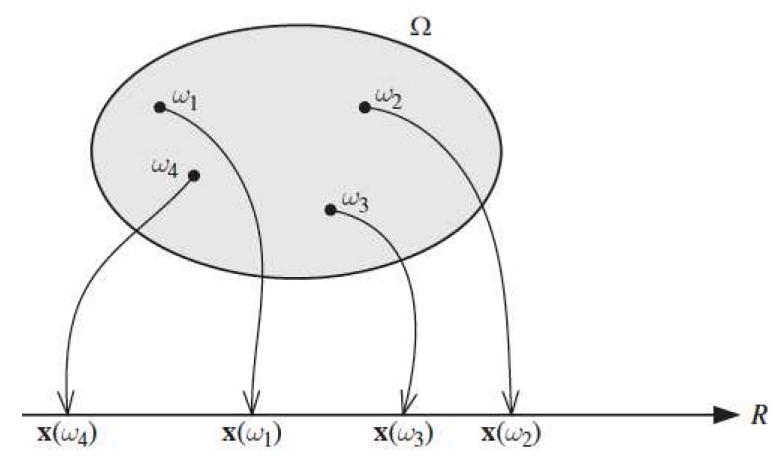
\includegraphics[width=5cm]{randomvariables}
		\caption{example of a random variable being mapped from a sample space $\Omega$ to a continuous set of the real number.}
	\end{SCfigure}
	
	To completely describe a random variable it's necessary to use a probabilistic description, in particular by using the so called \textbf{probability density function} (pdf) that can calculate the probability of a random variable $x$ at a certain value $x=a$ by the formula
	\[ p(a) = \lim_{\delta_a \rightarrow 0} \frac{\prob{a-\delta_a < x \leq a}}{\delta_a} \geq 0 \]
	This expression resembles a derivative: this function can in fact be integrated between two points in order to get the probability of having a random variables inside that range
	\[ \prob{a< x \leq b} = \int_a ^b p(x)\, dx \]
	From the probability density function it can be derived the \textbf{cumulative distribution function} (cdf) that describes the probability of having a random variable $x$ with value less or ugual to $b$:
	\[ P(b) = \prob{x\leq b} = \int_{-\infty}^b p(x)\, dx\]
	
	The pdf associated to a random variable, in order to satisfy the second axiom of probability, must require that
	\[ \prob{x\leq \infty} = \int_{-\infty}^\infty p(x)\, dx = P(\infty) = 1\] 
	\vspace{3mm}
	
	Usually all the probability density functions for continuous random variables can be expressed as a \textit{known distribution} by re-shaping the pdf as
	\[ p(x) = \frac{1}{c\, N(s)} p\left(\frac{x-l}{c}\right)\]
	where $l$ is the \textit{location parameter} (that has the role to translate the pdf), $c$ is the \textit{scale parameter} (associated to a expansion/contraction) and $s$ is a \textit{shape parameter} that governs the shape of the pdf and that define the normalising function $N(s)$.\\
	Examples of known probability density functions is the \textbf{uniform} one; in this case the random variable $x$ comparable to this distribution in the range $[a,b]$ is written as $x\backsim \mathcal U(a,b)$ and in particular
	\[ p(x) = \mathcal U(x; a,b) := \begin{cases}
		\frac 1{b-a} \qquad & \textrm{if } x\in [a,b] \\ 0 & \textrm{otherwise}
	\end{cases} \]
	Another important distribution is the \textbf{normal} $\mathcal N$ (or \textbf{gaussian}) one that requires the definition of all the 3 parameters defined above ($l, c,N(s)$) and the pdf associated is described as
	\[ p(x) = \mathcal N\big(x; l, c, N(s)\big) := \frac{1}{\sqrt{2\pi} c} e^{-\dfrac{(x-l)^2}{2c^2}} \]
	where $N(s)$= $\sqrt{2\pi}$ comes from the normalization of the pdf.
	\vspace{3mm}
	
	The analogous of the pdf for discrete valued variable $a$ is called \textbf{probability mass function} usually described as $\pi(a_i) = \prob{x=a_i} = \pi_i$. Knowing that the random variable has $n$ discrete steps, the following rule must be respected
	\[\sum_{i=1}^n \pi_i = 1\]
	An example of a probability mass function is the \textbf{Poisson} distribution with rate $\lambda$ that's used to calculate the probability of a certain number of random points in an interval $T$:
	\[ \pi(a) = \prob{x=a} = e^{-\lambda t} \frac{\big(\lambda T\big)^a}{a!} \qquad a \in \mathds N_0 \]
	\vspace{3mm}
	
	It is sometimes needed to characterise a random variable with certain attributes like the typical value, the spread or variability od the variable, and so on: this properties are computed on the probability density function of the variable, not non the raw collected data.\\
	In general we might be interested to calculate the \textbf{central value} of a random variable, but this value is'n unique and it depends on the definition adopted
	\begin{itemize}
		\item the \textbf{mode} corresponds to the value associated at the maximum of the pdf, so the most recurring value in the random variable domain; this central value definition isn't the best because in some cases it's possible to have multiple peaks;
		
		\item another way to determine the central value is by using the \textbf{moments} (concept derived by the mechanical world) calculating the $r-th$ moment with respect to the origin $\mu_r'$ or in respect to the mean $c_r'$ (in this case $\mu_1'$ is the mean value of the distribution):
		\[ \mu_r' = \int_{-\infty}^\infty x^r\, p(x)\, dx \qquad c_r' = \int_{-\infty}^\infty \big(x-\mu_1'\big)^r p(x)\, dx \]
		More precisely the moments are defined using the \textbf{expected value} operator $E(x)$ that's defined as
		\[ E(x) := \int_{-\infty}^\infty x p(x)\, dx\]
		By this new definition the $r-th$ moments of the random variables can be expressed as $\mu_r' = E\{x^r\}$ and $c_r' = E \big\{ (x-\mu_1')^r \big\}$. In particular for $r = 0$ no information are retrieved because for each random variable $x$ it happens that $\mu_0' = c_0' = 0$. By choosing $r = $, the value $\mu_1' := \mu$ represent the \textbf{mean} of the random variable, so \textit{the long run average}; calculating the value $c_1'$ gives no additional information ($c_1' = 0 \forall x$). By computing the $2-th$ moment it's possible to define the \textbf{variance} as $\sigma^2 := c_2'$.
	\end{itemize}

	So in general given a random variable $x$ it's possible to compute the mean $\mu$ and the variance $\sigma^2$ by using the following rules:
	\[ \mu = \int_{-\infty}^\infty x p(x)\, dx \qquad \sigma^2 = \int_{-\infty}^\infty \big(x-\mu \big)^2 p(x)\, dx  \]
	Applying this rule to the distributions mentioned before we can calculate the mean and the variance of a uniform distribution $\mathcal U (a,b)$ as $\mu = \frac{b+a}{2}$ and $\sigma^2 = \frac 1 {12} (b-a)^2$. Considering instead the gaussian distribution, the expected value is more complex to calculate, but some step of the demonstration are here described as well as the solution
	\begin{align*}
		E\{x\} = \mu & = \int_{-\infty}^\infty x \frac 1 {\sqrt{2\pi} c} e^{-\frac{(x-l)^2}{2c^2}} \, dx \\ & = \int_{-\infty}^\infty \big(x-l\big) \frac 1 {\sqrt{2\pi} c} e^{-\frac{(x-l)^2}{2c^2}} \, dx + l \int_{-\infty}^\infty x \frac 1 {\sqrt{2\pi} c} e^{-\frac{(x-l)^2}{2c^2}} \, dx \\
		& = \int_{-\infty}^\infty y \frac 1 {\sqrt{2\pi} c} e^{-\frac{y^2}{2c^2}} \, dy + l\\
		& = \int_{-\infty}^0 y \frac 1 {\sqrt{2\pi} c} e^{-\frac{y^2}{2c^2}} \, dy + \int_0^\infty y \frac 1 {\sqrt{2\pi} c} e^{-\frac{y^2}{2c^2}} \, dy + l \\
		& = l
	\end{align*}
	So in this case it's possible to see that the mean of a normal distribution is equal to the location parameter $l$ described by the function, and (as it's going to be demonstrated) the variance is equal to the scale parameter $\sigma^2 = c^2$:
	\begin{align*}
		V\{x\} = \sigma^2 & = E\big\{(x-\mu)^2\big\} = \int_{-\infty}^\infty \big(x-\mu\big)^2 \frac 1 {\sqrt{2\pi} c} e^{-\frac{(x-\mu)^2}{2c^2}} \, dx \\
		& = \int_{-\infty}^\infty y^2 \frac 1 {\sqrt{2\pi} c} e^{-\frac{y^2}{2c^2}} \, dx = c^2
	\end{align*}
	In general the value $\sigma= \sqrt{\sigma^2}$ is defined as \textbf{standard deviation}. In a practical way the mean value gives an idea of the central value of the random variable while the variance represent how much this variable is spread.
	
	Another important way to determine the central value is by computing the \textbf{median} $\tilde \mu$ of a random variable, so by determining the values that satisfies the following equation:
	\[ \int_{-\infty} ^{\tilde \mu} p(x)\, dx = \int_{\tilde \mu}^\infty p(x) \, dx \]
	In general the median is a more robust way to estimate the central value of a random variable and so it's often more used; direct consequence of the median is the \textbf{mean deviation} (concept that replaces the variance) defined as
	\[ \overline \mu = \int_{-\infty}^\infty |x-\mu| p(x)\, dx \]
	
	
	
	
	
	
	
	
	
	
	
	
	
	
	
	
	
	
	
	
	
	
\end{document}